\documentclass[conference]{IEEEtran}
\usepackage{cite}
\usepackage{amsmath,amssymb,amsfonts}
\usepackage{algorithmic}
\usepackage{graphicx}
\usepackage{textcomp}
\usepackage{xcolor}
\def\BibTeX{{\rm B\kern-.05em{\sc i\kern-.025em b}\kern-.08em
    T\kern-.1667em\lower.7ex\hbox{E}\kern-.125emX}}
\begin{document}

\title{100W Low Voltage AC-DC Converter\\}


\author{\IEEEauthorblockN{Chasen Gaither}
\IEEEauthorblockA{\textit{Student ID: 1974745} \\
\textit{University of Washington}\\
Seattle, WA, USA \\
chasennn@uw.edu}
\and
\IEEEauthorblockN{Khushbu Patel}
\IEEEauthorblockA{\textit{Student ID: 2400367} \\
\textit{University of Washington}\\
Seattle, WA, USA \\
kbupatel@uw.edu}
\and
\IEEEauthorblockN{Enrique Antunano}
\IEEEauthorblockA{\textit{Student ID: 2400331} \\
\textit{University of Washington}\\
Seattle, WA, USA \\
enriantu@uw.edu}
}

\maketitle

\begin{abstract}
This document covers the design of a DO-160G EMI Category L, M, H compliant AC-DC converter that accepts an input voltage of 115 \textit{Vac}, 400 \textit{Hz}, 
and can provide up to an output voltage of 100 \textit{W} at 28 \textit{Vdc}.
\end{abstract}

\section{Introduction}
This document covers the design of a DO-160G EMI compliant AC-DC converter that accepts a 115 \textit{Vac}, 400 \textit{Hz}, voltage input
and can provide up to 100 \textit{W} to a 28 \textit{Vdc} output. The power path will require AC rectification and a DC step-down with a buck converter. As the team's experience is in the aerospace industry, DO-160G EMI requirements will be used instead of FCC or CISPR requirements. DO-160G covers the compliance of aircraft equipment with multiple environmental and electromagnetic conditions found in aircraft. DO-160G is referenced by the FAA’s Advisory Circular AC 21-16G and other regulatory authorities worldwide. The team decided to pursue an aerospace standard since all three team members work in the aerospace industry and find the experience invaluable for their own professional growth.

\section{EMI Compliance Standard}

The team will adhere to the DO-160G design standard for Category L, M, and H electronics. DO-160G is maintained by the Radio Technical Commission for Aeronautics (RTCA). Category L, M, and H cover electronics that are far from apertures of an aircraft, near apertures, and direct view of RF antennas of an aircraft. Given the time constraints of this course and knowledge breadth across the team, the design the AC-DC converter adheres to the stricter EMI emissions limit without going to the extreme of the DO-160G standard. As reference, category B is the least strict, categories L,M, and H are in the middle, and categories P and Q are the most strict. Additionally, the team will focus primarily on modeling the power rail behavior and ignore the EMI limits specified for Interconnecting Bundles.

\subsection{Conducted Emissions Requirement}

Conducted Emissions requirements are specified in RTCA / DO-160 Conducted Emissions testing, Section 21.0. The test's range of interest goes from 150${kHz}$ to 152${MHz}$.

See Figure \ref{fig:do-160g_conducted_emissions_limit_diagram} for a graph of the conducted emission limit for categories L, M, and H for power lines.

\begin{figure}[htbp]
    \centering
    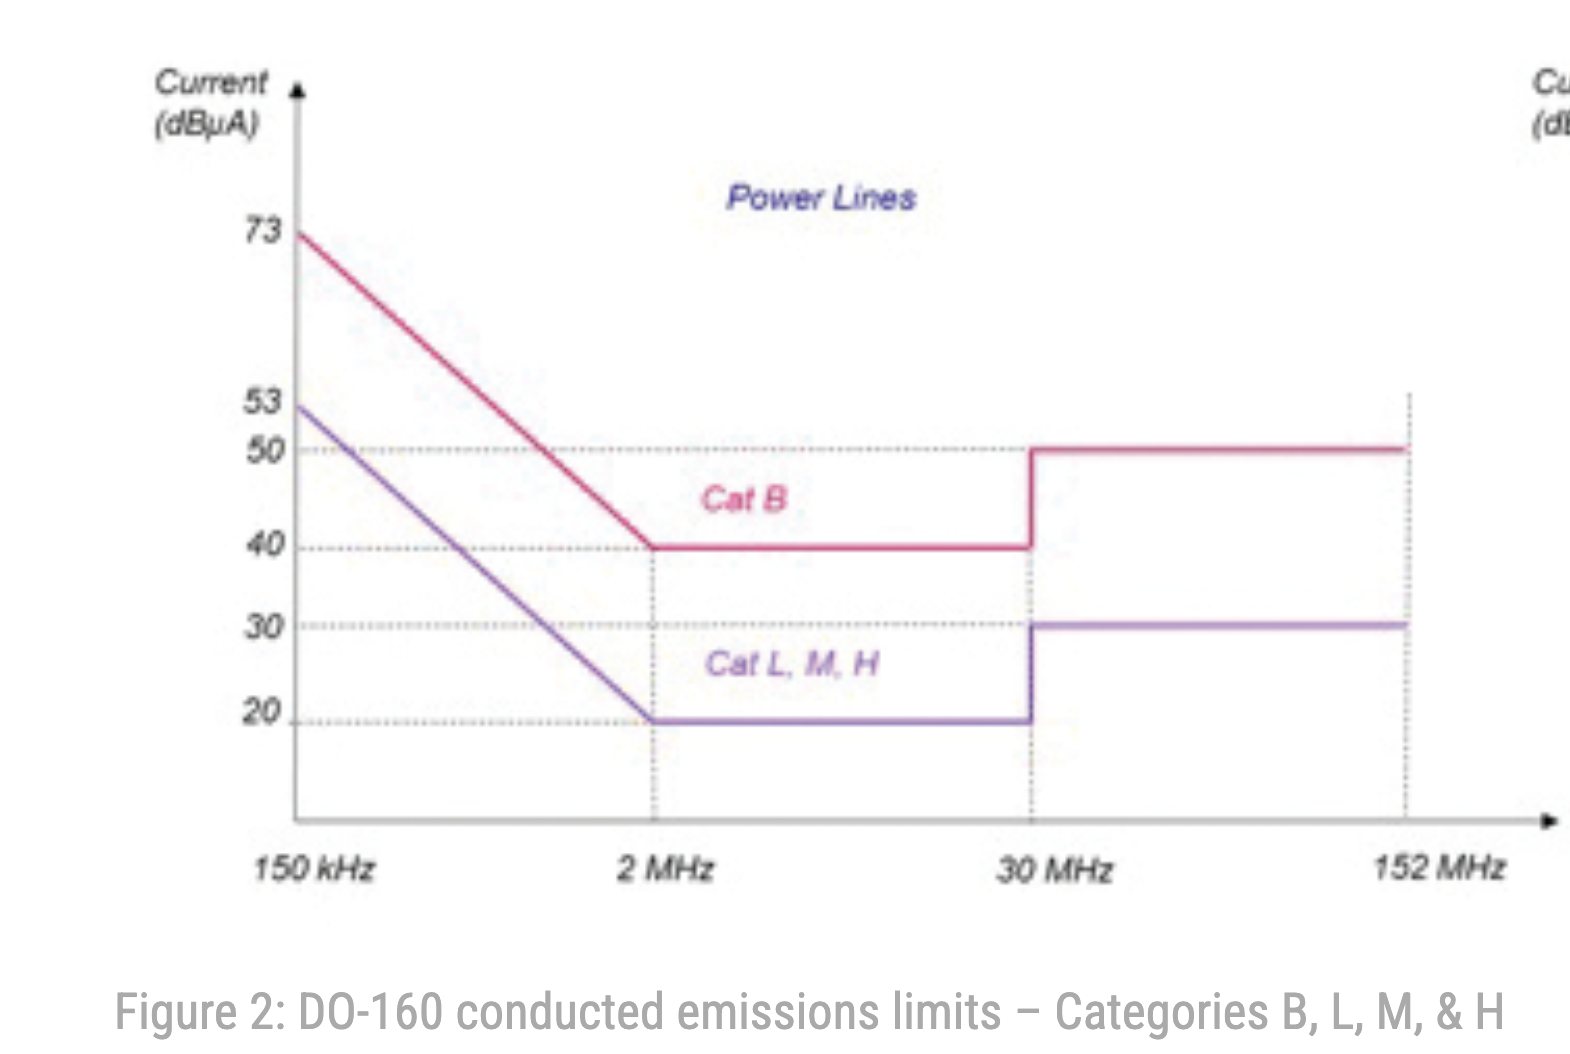
\includegraphics[width=1.0\linewidth]{do-160g_conducted_emissions_limit.png}
    \caption{DO-160G Conducted Emissions Limit for Category L, M, and H for Power Lines}
    \label{fig:do-160g_conducted_emissions_limit_diagram}
\end{figure}

\subsection{Direct Lightning Pin Injection Requirement}
Lightning induced transient susceptibility requirements are specified in RTCA / DO-160 Direct Lightning Pin Injection testing, Section 22.0. Indirect lightning testing will not be conducted, as these test requirements are for transient injection at the cable bundle, and the focus of this project is on the power rail of the equipment-under-test (EUT). Compliance will be conducted through LTSpice simulation of test injection waveforms specified by DO-160G, which provide a representation of a lightning strike. Direct pin injection testing for this project will be done with waveform set A, see Figure \ref{fig:do-160f_pin_injection_test_table} for the waveforms called out by set A. Set A will be used because set B specifies injection at a cable bundle rather than at the EUT pin. 

\begin{figure}[hp]
    \centering
    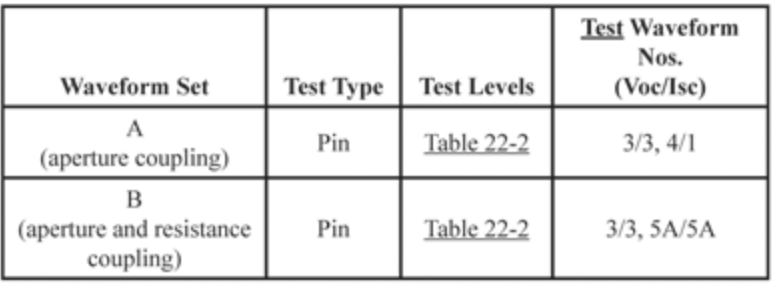
\includegraphics[width=1.0\linewidth]{do-160f_pin_injection_test_table.png}
    \caption{DO-160F Direct Pin Injection Lightning Test Table}
    \label{fig:do-160f_pin_injection_test_table}
\end{figure}

Set A's waveform 3 injects a damped oscillatory voltage and current waveform. See Figure \ref{fig:do-160f_waveform_set_3_diagram} for the waveform.

\begin{figure}[hp]
    \centering
    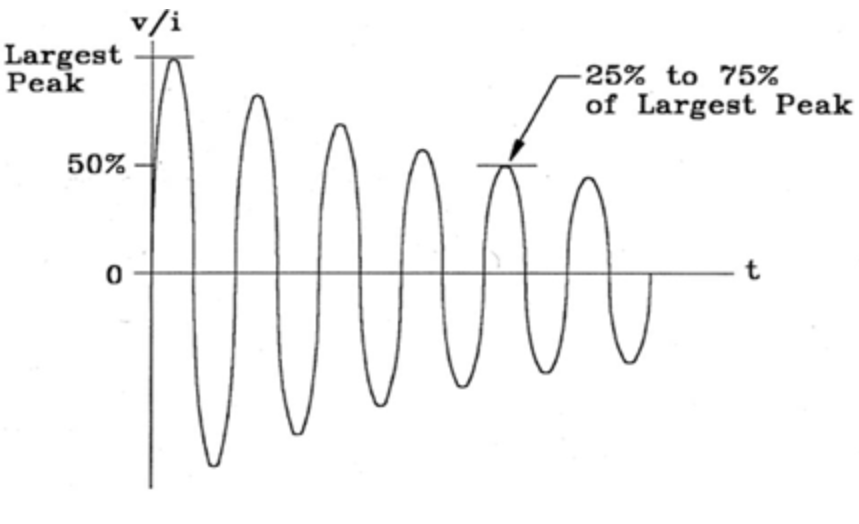
\includegraphics[width=1.0\linewidth]{do-160f_waveform_set_3.png}
    \caption{DO-160F Direct Pin Injection Lightning Test Waveform 3}
    \label{fig:do-160f_waveform_set_3_diagram}
\end{figure}

Set A's waveform 4 injects a peak voltage that peaks according to a time variable ${T1}$ and decays to 50\% of $V_{peak}$ by time ${T2}$. See Figure \ref{fig:do-160f_waveform_set_4_diagram} for the waveform.

\begin{figure}[hp]
    \centering
    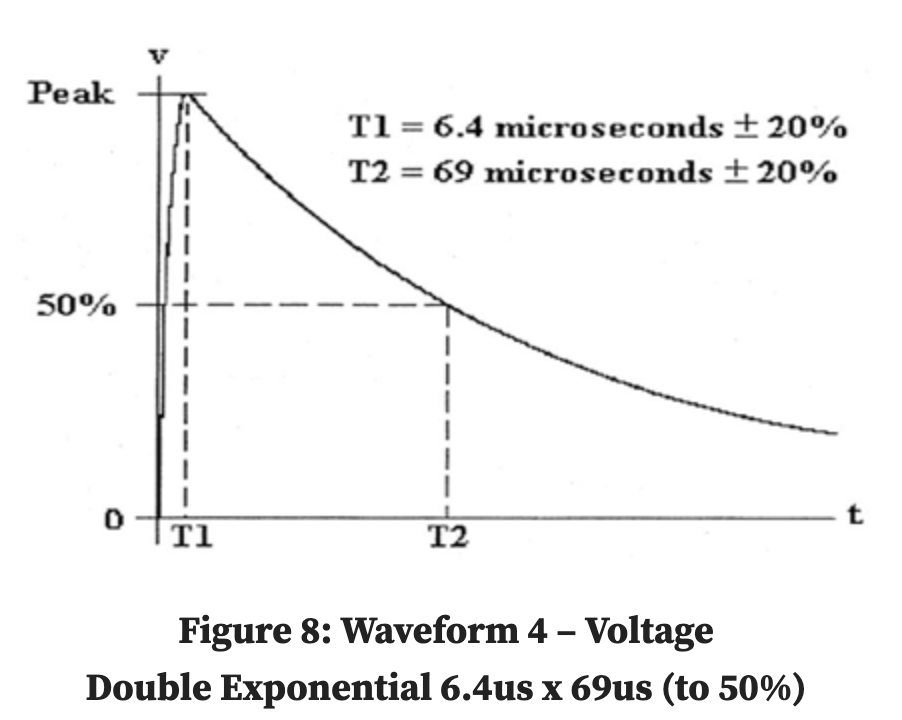
\includegraphics[width=1.0\linewidth]{do-160f_waveform_set_4.png}
    \caption{DO-160F Direct Pin Injection Lightning Test Waveform 4}
    \label{fig:do-160f_waveform_set_4_diagram}
\end{figure}

\section{Circuit Architecture}

\subsection{High-Level Overview}

Figure \ref{fig:ac_dc_converter_ideal_diagram} presents a high-level overview of an ideal AC-DC converter. The team opted to implement a modified 115$V_{AC}$ - 28$V_{DC}$ AC-DC converter that removed the transformer from the circuit as shown in Figure \ref{fig:ac_dc_converter_implemented_diagram}. Although an AC-DC converter may typically include a transformer to reduce common-mode noise when stepping down the $V_{AC}$, the team decided to eliminate the component to increase noise within the circuit's power path and instead, demonstrate the impact that proper filtering would have on load voltage and current. In practical applications found in the industry, if size and weight were not constraints, then a transformer would likely be included.

\begin{figure}[htbp]
    \centering
    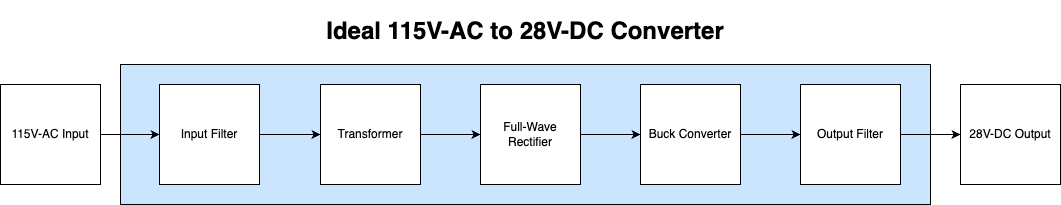
\includegraphics[width=1.0\linewidth]{ac_dc_converter_ideal.png}
    \caption{Ideal AC-DC Converter}
    \label{fig:ac_dc_converter_ideal_diagram}
\end{figure}

\begin{figure}[h]
    \centering
    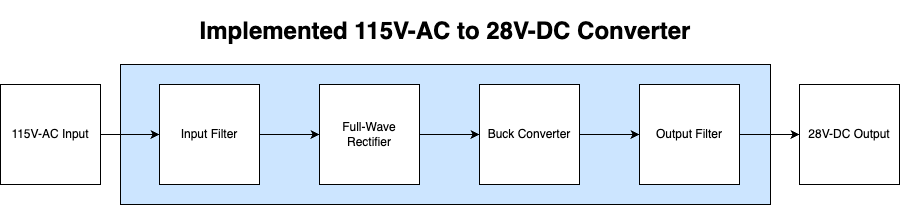
\includegraphics[width=1.0\linewidth]{ac_dc_converter_implemented.png}
    \caption{Implemented AC-DC Converter}
    \label{fig:ac_dc_converter_implemented_diagram}
\end{figure}

\subsection{Input Filter}

The input filter consists of two sub-circuits: (1) a pair of line-to-chassis ground capacitors and (2) a pair of RLC filters. The line-to-chassis ground Y-capacitors handle common-mode noise from the 115$V_{AC}$ input rail. Meanwhile, the two RLC circuits stabilize the voltage input of the full-wave rectifier. The two RLC circuit design, one per power rail, is borrowed from common industry best practices. Based on simulations, two RLC circuits moved the peak AC voltage down versus a single RLC circuit block. The trade-off between the inclusion of the damping resistors versus increased power consumption is okay for the main objectives of the project. Based on simulations, there was very little common-mode noise on the input of the 115$V_{AC}$ to 28$V_{DC}$, so no common-mode was included in the design. Refer to Figure \ref{fig:input_filter_top_level_diagram} for the top-level design of the input filter. 

\begin{figure}[htp]
    \centering
    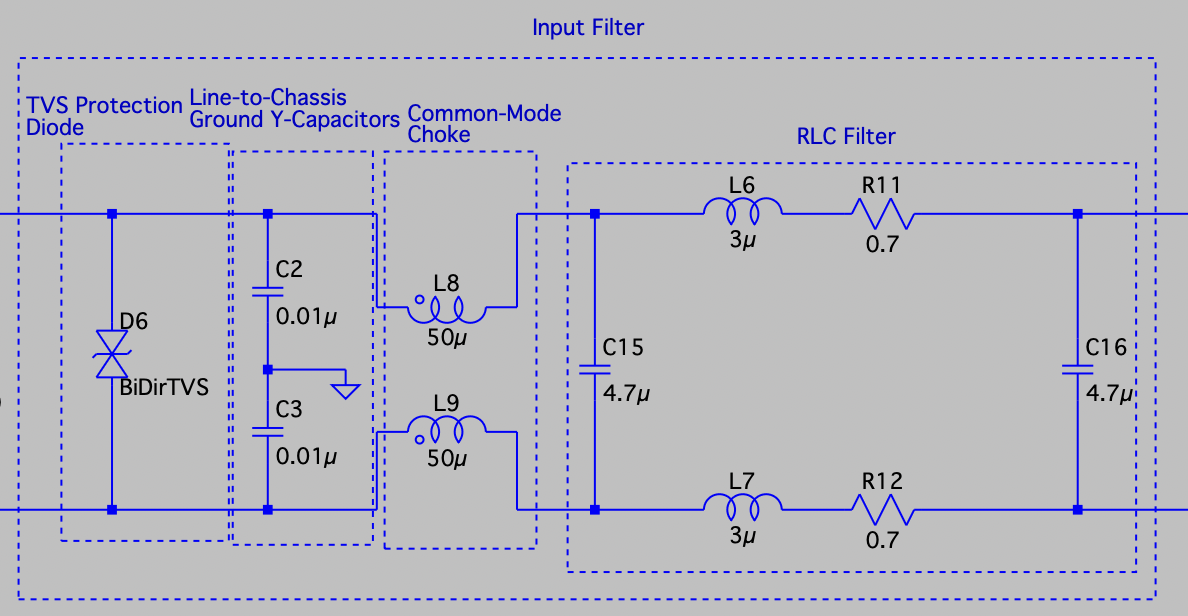
\includegraphics[width=1.0\linewidth]{input_filter_top_level.png}
    \caption{Input Filter Top Level}
    \label{fig:input_filter_top_level_diagram}
\end{figure}

\subsection{Full-Wave Bridge Rectifier}
Directly after the AC input filters, the AC signal is fed into a full-wave bridge rectifier. The function of a full-wave rectifier is to convert the positive and negative half-cycles of an AC signal into a pulsating DC signal output, see Figure \ref{fig:full-wave_rectifier_output_waveform_diagram}. From there, a bulk capacitor is used on the output to "smooth" out the pulsating DC signal so that the output signal begins to resemble a stable DC output, see Figure \ref{fig:full-wave_bridge_rectifier_filter_waveform_diagram}. 

\begin{figure}[htp]
    \centering
    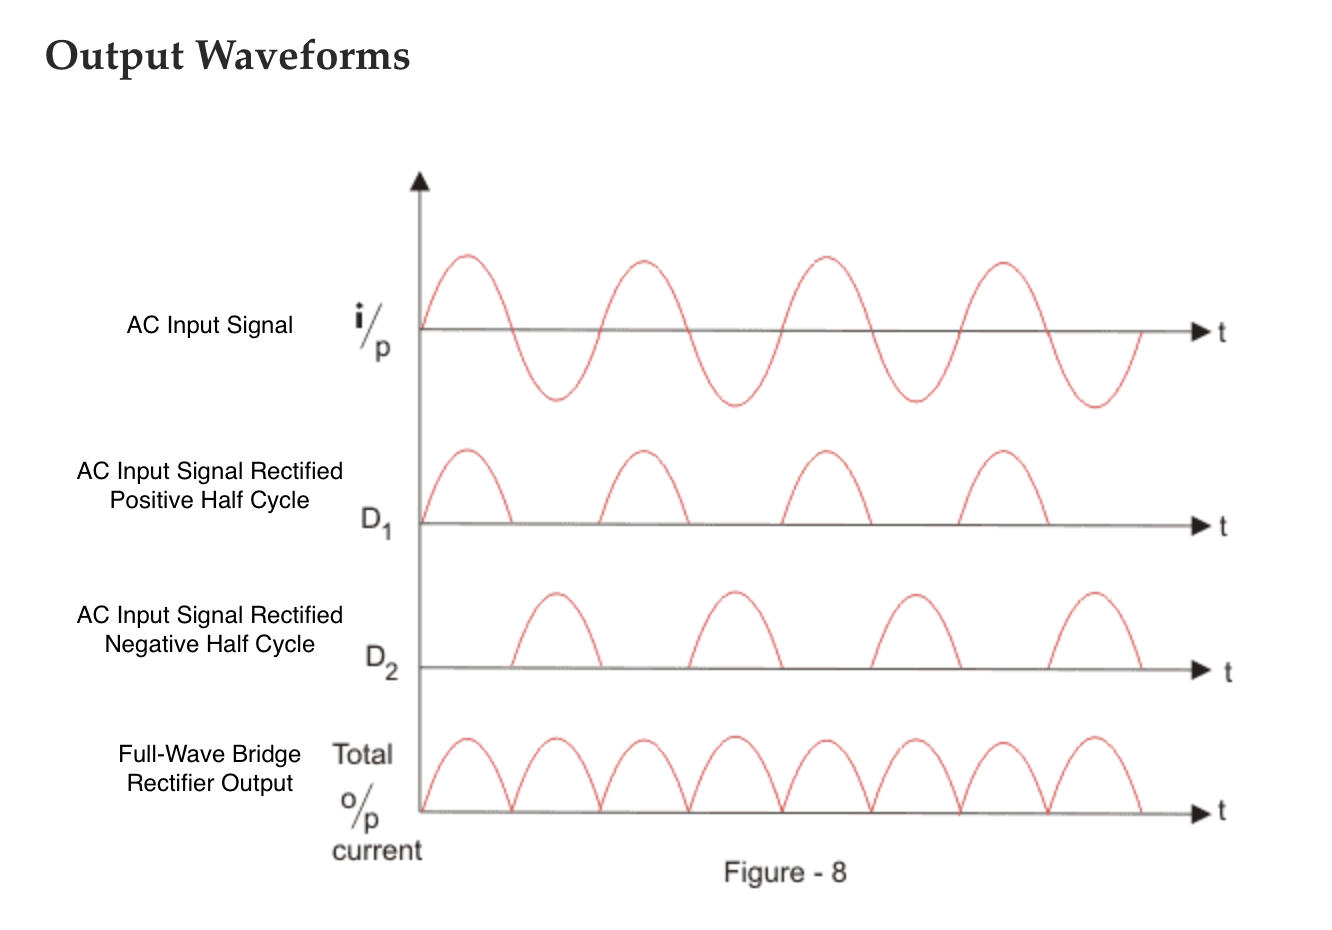
\includegraphics[width=1.0\linewidth]{full-wave_bridge_rectifier_output_waveform.png}
    \caption{Full-Wave Rectifier Output Waveforms}
    \label{fig:full-wave_rectifier_output_waveform_diagram}
\end{figure}

\begin{figure}[h]
    \centering
    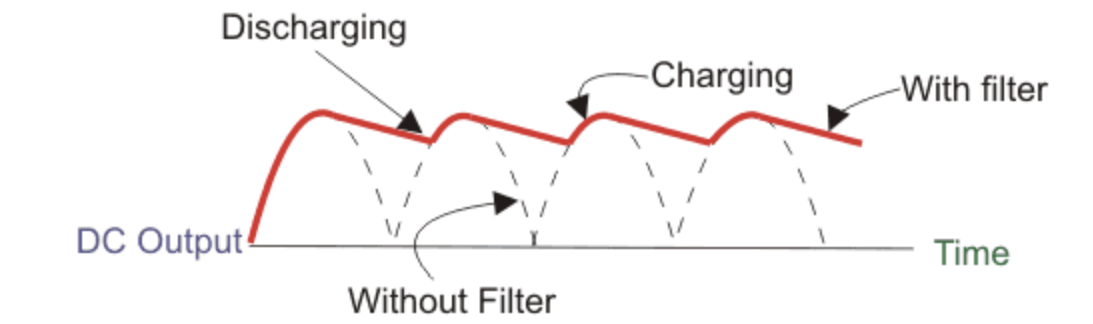
\includegraphics[width=1.0\linewidth]{full-wave_bridge_rectifier_filter_waveform.png}
    \caption{Full-Wave Rectifier Filter Waveform}
    \label{fig:full-wave_bridge_rectifier_filter_waveform_diagram}
\end{figure}


A full-wave bridge rectifier was implemented because of its efficiency in comparison to a half-wave rectifier. The LTSpice model is shown in Figure \ref{fig:full-wave_bridge_rectifier_circuit_diagram}. For a full-wave rectifier, both cycles of the AC signal are converted into the DC signal. For a half-wave rectifier, only a single half cycle of the AC signal is transferred, while the other half cycle is blocked. 

\begin{figure}[htp]
    \centering
    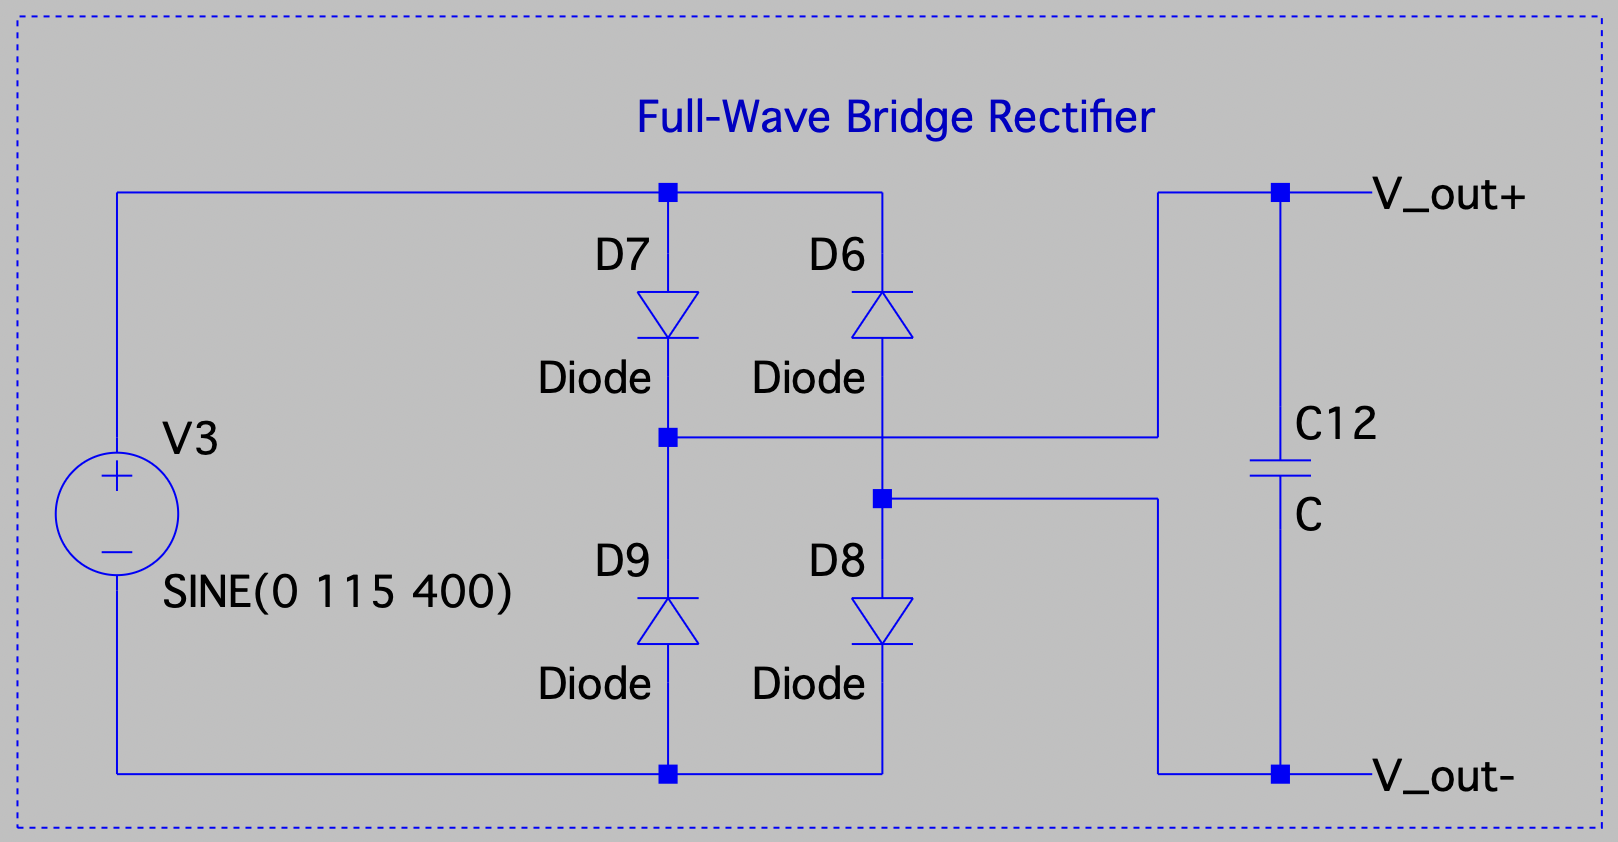
\includegraphics[width=1.0\linewidth]{full-wave_bridge_rectifier_circuit.png}
    \caption{Full-Wave Bridge Rectifier Circuit}
    \label{fig:full-wave_bridge_rectifier_circuit_diagram}
\end{figure}

\subsection{Buck Converter}
After the full-wave bridge rectifier is a Buck Converter. A buck converter is a DC-DC converter that steps down the DC input voltage using a voltage-controlled switch to generate a PWM output. After the PWM output, there is a bulk LC filter. The primary purpose of the bulk inductor and capacitor is to generate a stable stepped down DC output from the switching regulator's PWM input voltage. High-frequency noise introduced by the switching regulator will be handled by a separate block of output filtering components rather than by the bulk inductor and capacitor components. See Figure \ref{fig:buck_converter_circuit_diagram} for a diagram of a buck converter circuit.

\begin{figure}[htp]
    \centering
    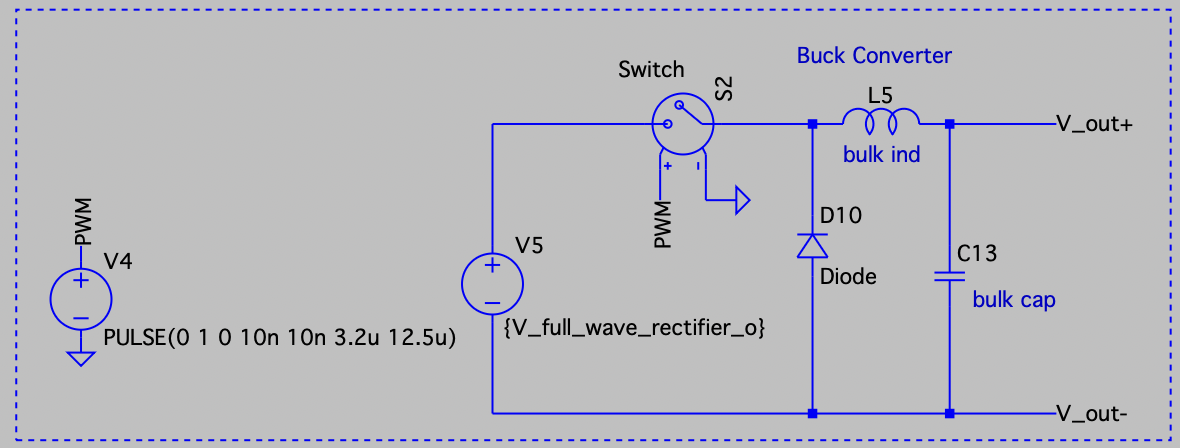
\includegraphics[width=1.0\linewidth]{buck_converter_circuit.png}
    \caption{Buck Converter Circuit}
    \label{fig:buck_converter_circuit_diagram}
\end{figure}

The bulk inductor resists changes in current, so when the switch is turned off, it attempts to keep the current constant. Meanwhile, the bulk capacitor resists changes in voltage, and thus attempts to keep the output voltage constant. The LC circuit includes a protection diode to prevent the switch from being damaged by a reverse voltage spike from the inductor's stored energy when the switch turns ON again. In contrast, when the switch is turned OFF, the forward bias of the protection diode allows the inductor to discharge its stored current. See Figure \ref{fig:buck_converter_waveform_diagram} for a diagram of the expected output waveforms of the buck converter.

\begin{figure}[htp]
    \centering
    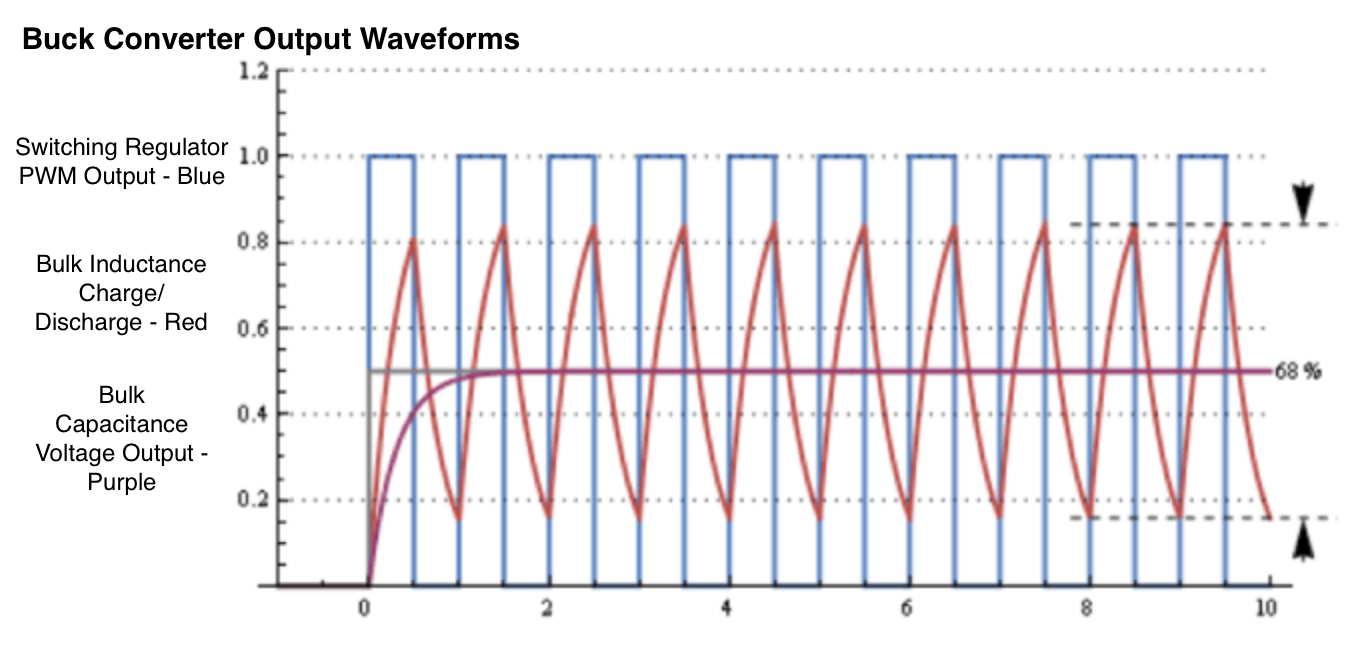
\includegraphics[width=1.0\linewidth]{buck_converter_waveform.png}
    \caption{Buck Converter Expected Output Waveform}
    \label{fig:buck_converter_waveform_diagram}
\end{figure}

The team decided to move away from a linear regulator because the circuit is not as power-efficient as a switching regulator. The drawback of using a switching regulator is the voltage ripple introduced onto the DC output power rail due to the switching frequency. The switching noise and its harmonics will require output filtering to minimize the voltage ripple seen by the load and to guarantee that the conducted emissions of our circuit are below the DO-160G EMI conducted emissions threshold. 

The switching voltage regulator will not use a feedback loop for auto-adjustment of the switch's duty cycle. For a power rail, typically a feedback loop would be used to adjust the switch's duty cycle so that the power rail can maintain a 28$V_{DC}$ output across a range of loads. The scope of this course focuses on EMI compliance and circuit design, so the 28$V_{DC}$ output will be optimized to meet the objective of 100$W$ power output in compliance with the DO-160G standard. If this were a power electronics course, then the team would have opted to design a feedback loop to the switching regulator so that the 115$V_{AC}$ to 28$V_{DC}$ converter would be complaint across loads.

\subsection{Output Filter}
The output filter for this current circuit design must suppress the noise introduced by the switching regulator in the 150${kHz}$ - 152${MHz}$ range, prevent common-mode noise from propagating to the load and from the load side, and eliminate differential-mode noise from the load. 

The output filter design is presented in Figure \ref{fig:output_filter_top_level_diagram}. The output filter consists of two stages of RLC filtering, followed by unit-side line-to-chassis ground Y-capacitors, a common-mode choke, and load-side line-to-chassis ground Y-capacitors. Each sub-circuit of the output filter will be further analyzed.

\begin{figure}[htp]
    \centering
    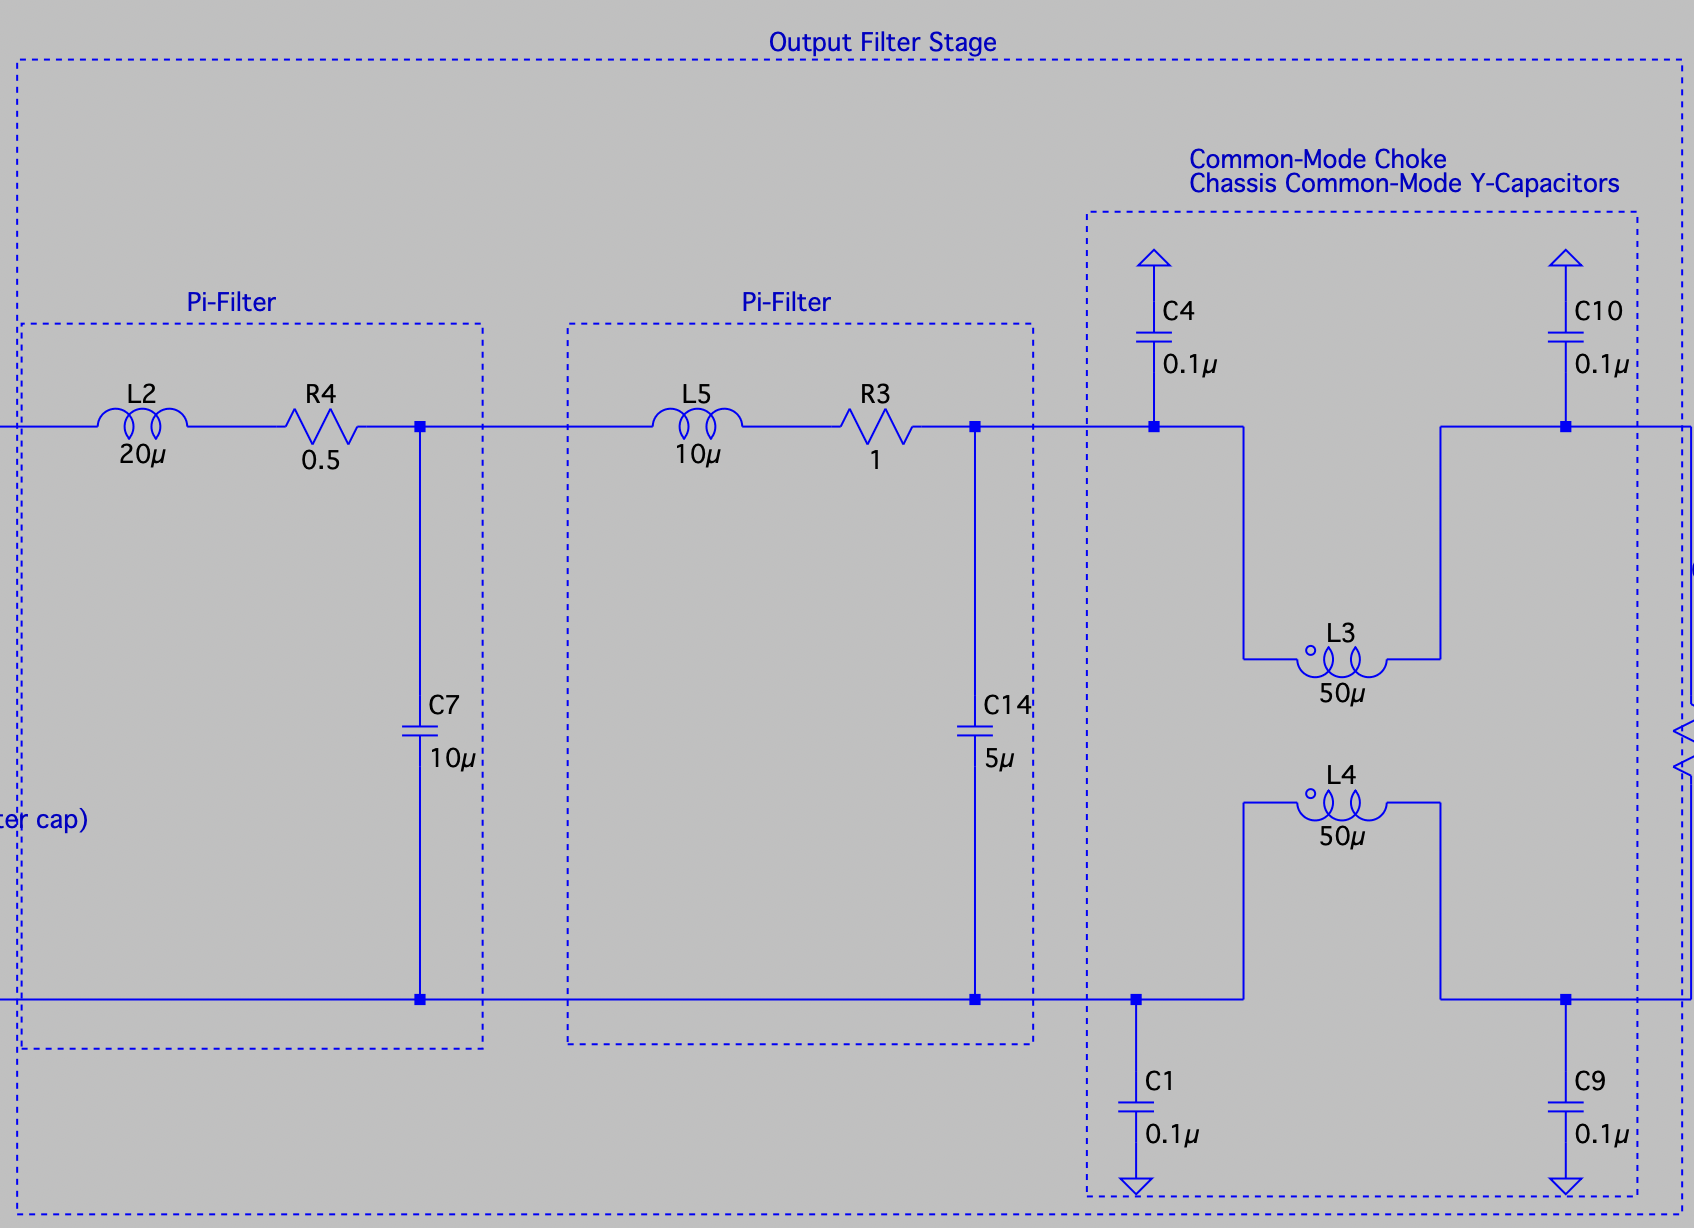
\includegraphics[width=1.0\linewidth]{output_filter_top_level.png}
    \caption{Output Filter Top-Level}
    \label{fig:output_filter_top_level_diagram}
\end{figure}

As part of the output filter deconstruction, two RLC filters implemented to attain -40${dB}$ attenuation of the high-frequency ripple voltage from the buck converter. The initial design of the output filter consisted of only one pi filter, but additional attenuation was required to meet the standard of conducted emissions DO-160G. The second design iteration consisted of two pi filters, but simulation showed that the higher value capacitor from one pi filter would dominate the other pi filter's capacitor. So, the pi filters were replaced with RLC filters.

RLC filters were chosen for their damping resistor. Damping was considered necessary for two reasons. First, although the noise across the load was below the DO-160G emissions line, the margin was 2${db}$ for a harmonic of the switching regulator noise. To increase the margin, an LC filter with a larger capacitor or inductance could have been applied. The risk of increasing the capacitance or inductance was that the LC filter's resonance was already in the middle of the AFCS range, and increasing the capacitor or inductor value does not eliminate our resonant frequency risk. So, a low value damping resistor is included to provide a sufficient damping factor (>1) while balancing power consumption by the set of damping resistors.

The second part of the output filter consists of a common-mode choke and Y-capacitors from rail-to-chassis ground on both the unit-side and load-side of the choke. From simulation, the common-mode noise was minimal, but we think it's good design practice to isolate the unit-side's common-mode noise and the load-side's common-mode noise.

\section{Simulation Setup}

\subsection{Input Filter}

\subsection{Full-Wave Bridge Rectifier}
To model the full-wave bridge rectifier in LTSpice, t

\subsection{Buck Converter}
\subsubsection{Buck Converter Power Efficiency Estimation}
\subsubsection{LC Filter Calculation}
\subsection{Output Filter}


\section{Results}
\subsection{Input Filter}

The input filter's RLC circuit, which lies between the full-wave bridge rectifier and the ac voltage source, forces the current across R2 to retain most of its ac sine wave characteristic. There are large current spikes on the ac input that occur as the signal oscillates, see Figure \ref{fig:ac_input_waveform}. The spikes are attributable to the diodes of the full-wave rectifier reaching their threshold voltage, which allows current to flow and charge the bulk capacitor of the full-wave bridge rectifier.

\begin{figure}[htp]
    \centering
    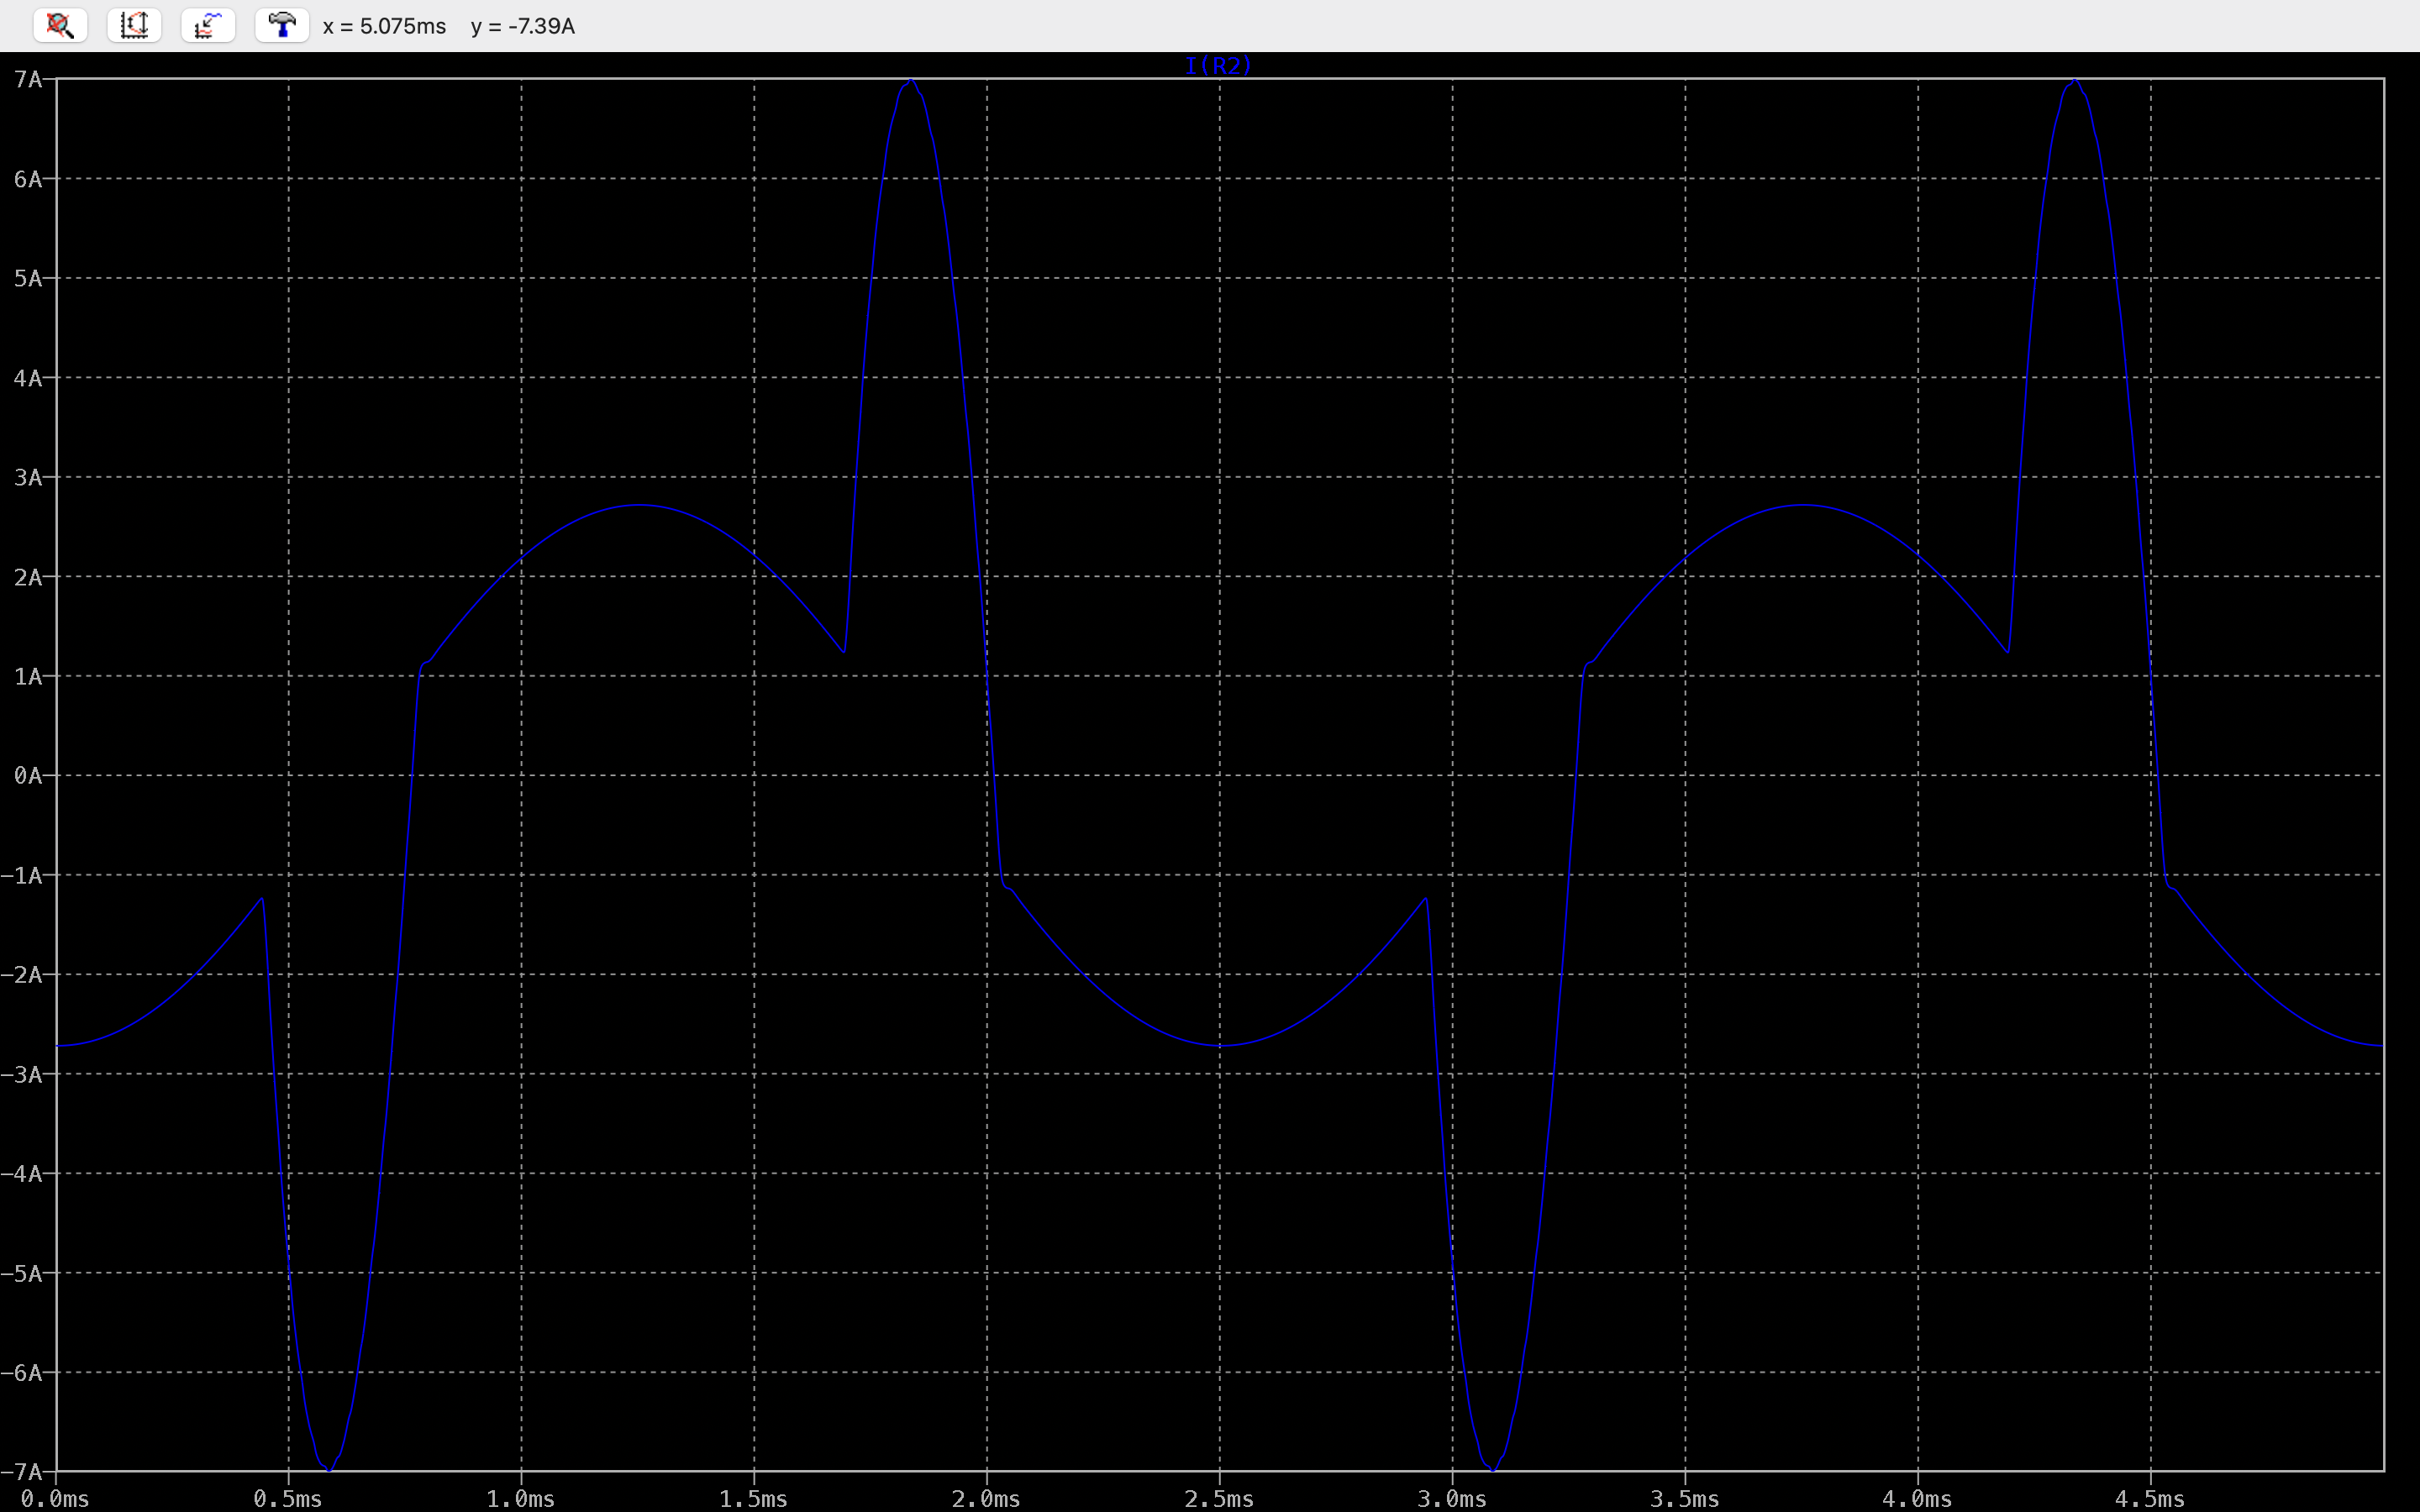
\includegraphics[width=1.0\linewidth]{ac_input_waveform.png}
    \caption{115$V_{AC}$ Input Waveform}
    \label{fig:ac_input_waveform}
\end{figure}

The common-mode noise from the ac input was very small and occurred when the diodes were enabled, see Figure \ref{fig:ac_input_common_mode_y_cap_noise_waveform}. The spike in current introduces noise into the circuit. The simulation shows that the small common-mode noise across the Y-capacitors, directly at the voltage source edge, is filtered out.

\begin{figure}[htp]
    \centering
    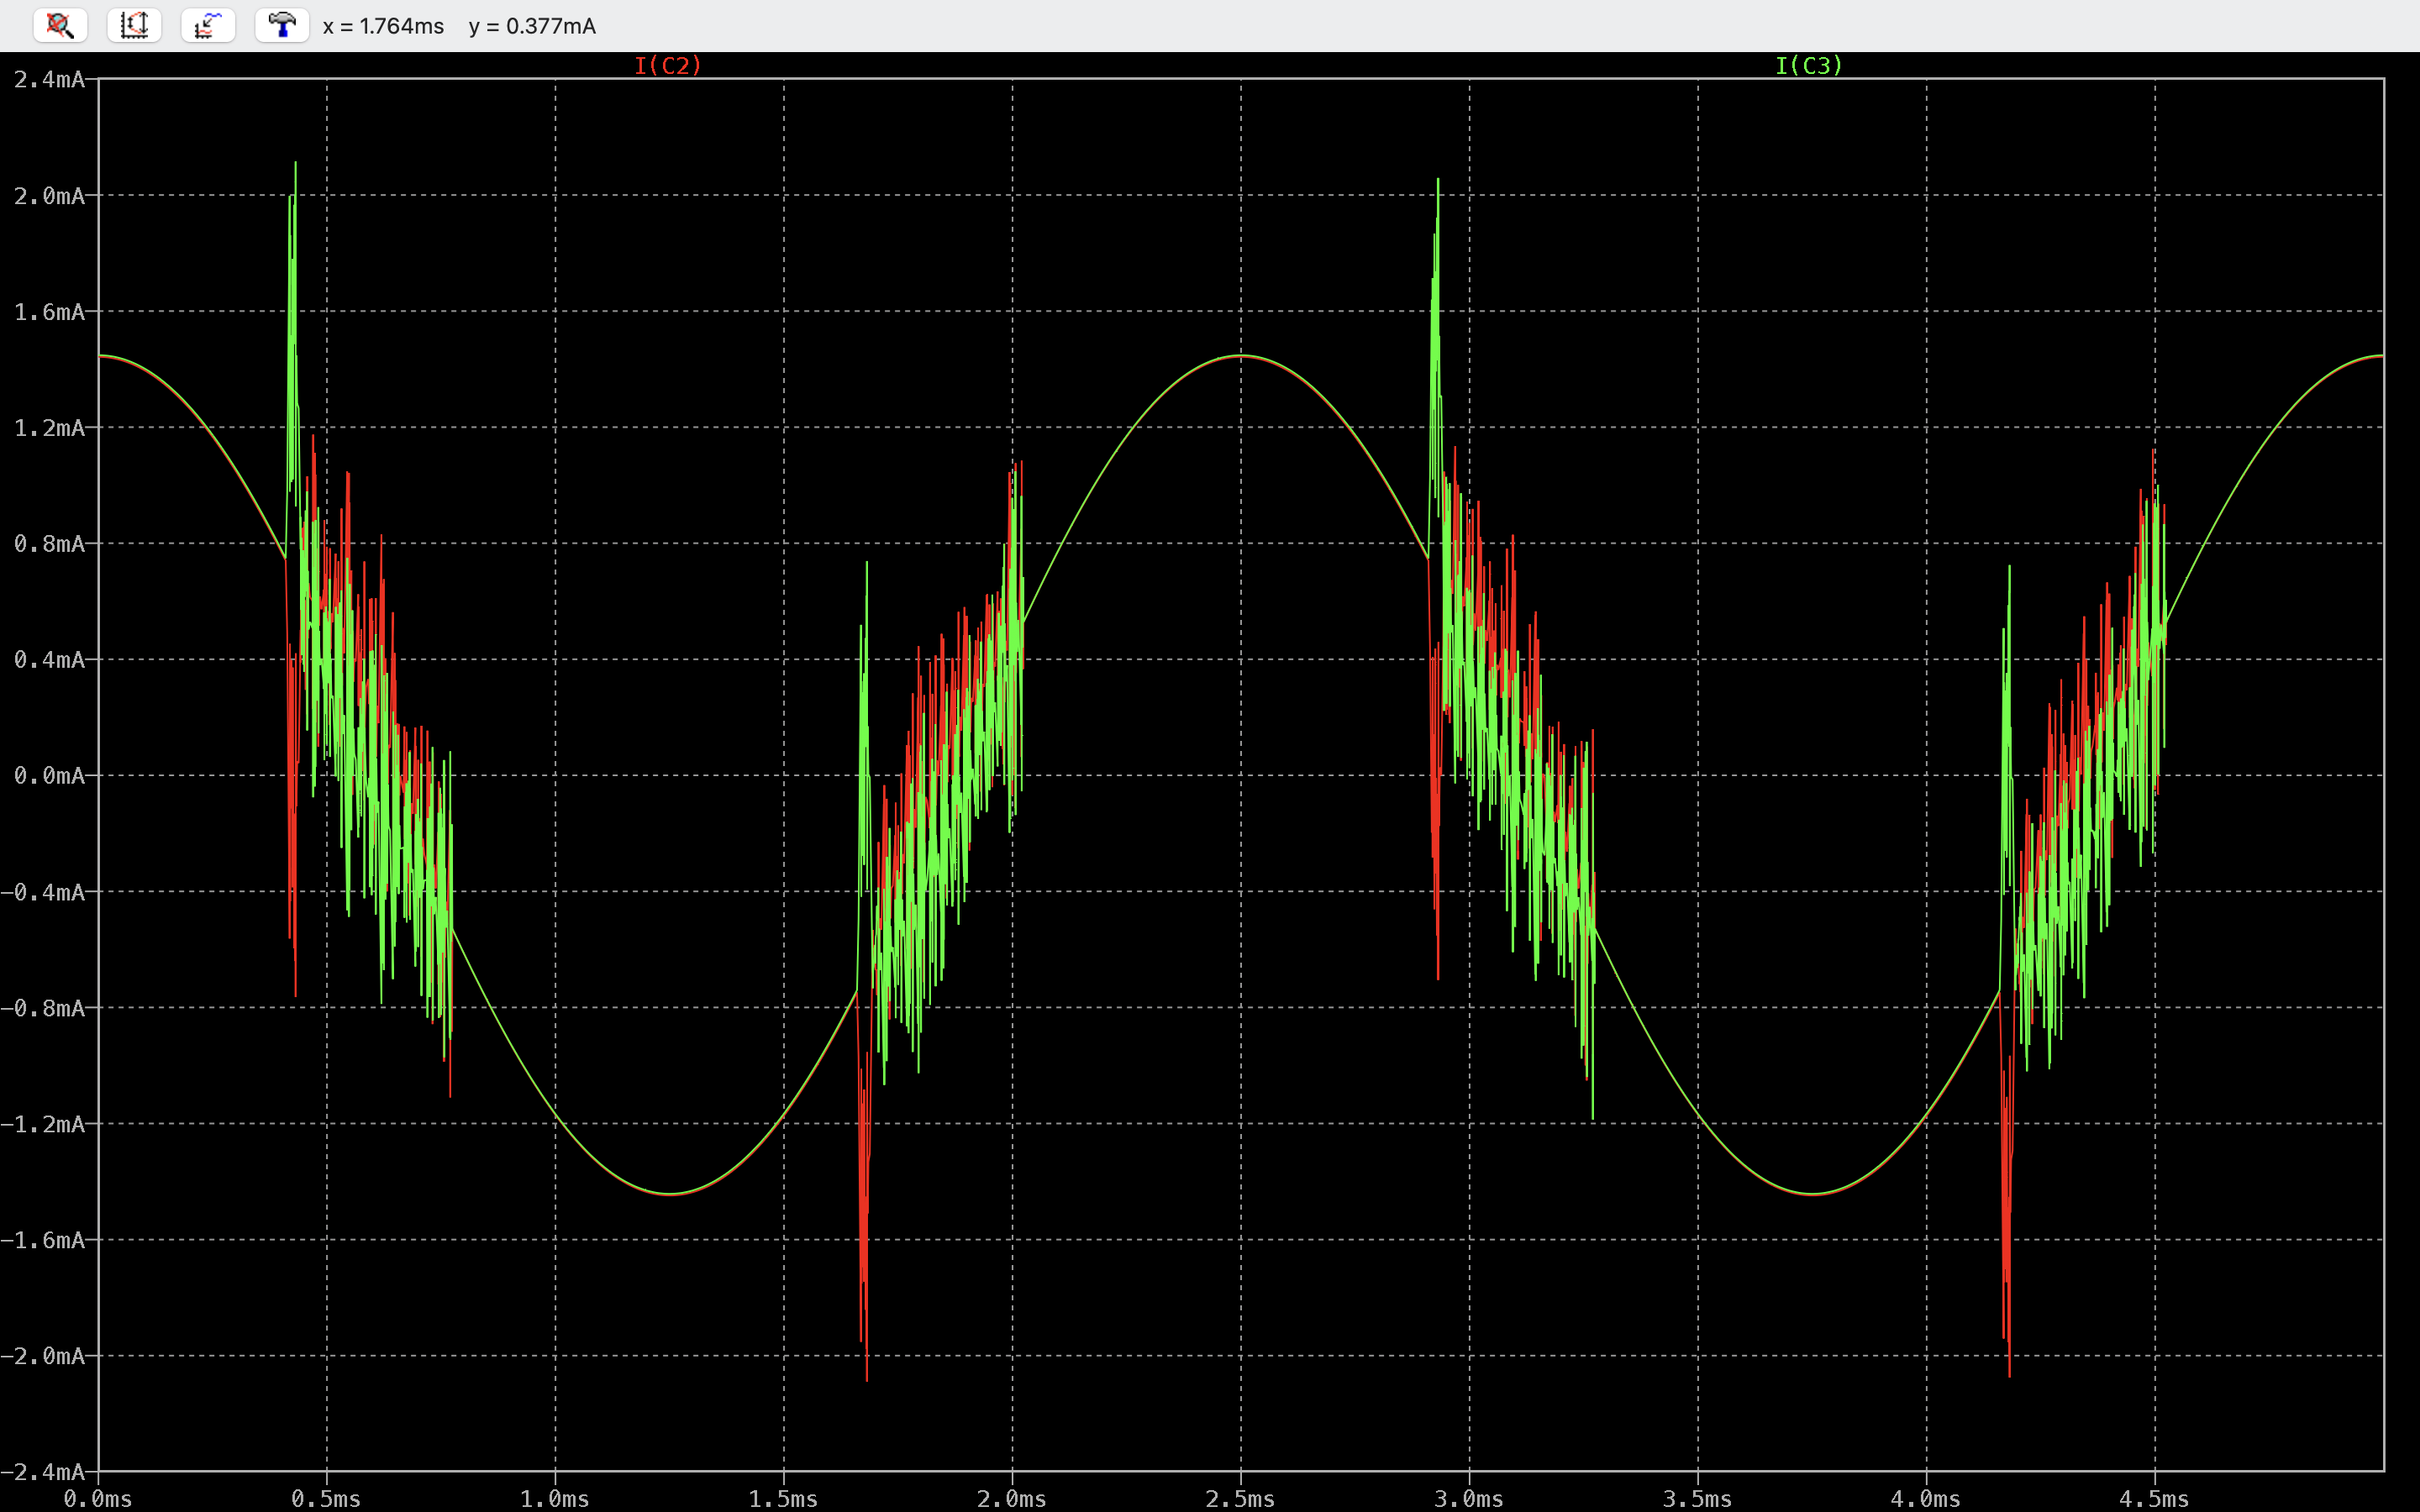
\includegraphics[width=1.0\linewidth]{ac_input_common_mode_y_cap_noise_waveform.png}
    \caption{Common-Mode Noise across Y-Capacitors on 115$V_{AC}$ Input Line}
    \label{fig:ac_input_common_mode_y_cap_noise_waveform}
\end{figure}

The current measurement across R11 demonstrates how the inductor, L6, resists changes in current from the 115 $V_{ac}$ source and smooths the input waveform. The current across the RLC's capacitor, C16, is high-frequency noise shunted to the negative rail. The current after capacitor C16, measured across $R5$, is a clean ac input, see Figure \ref{fig:ac_input_rlc_waveforms}

\begin{figure}[htp]
    \centering
    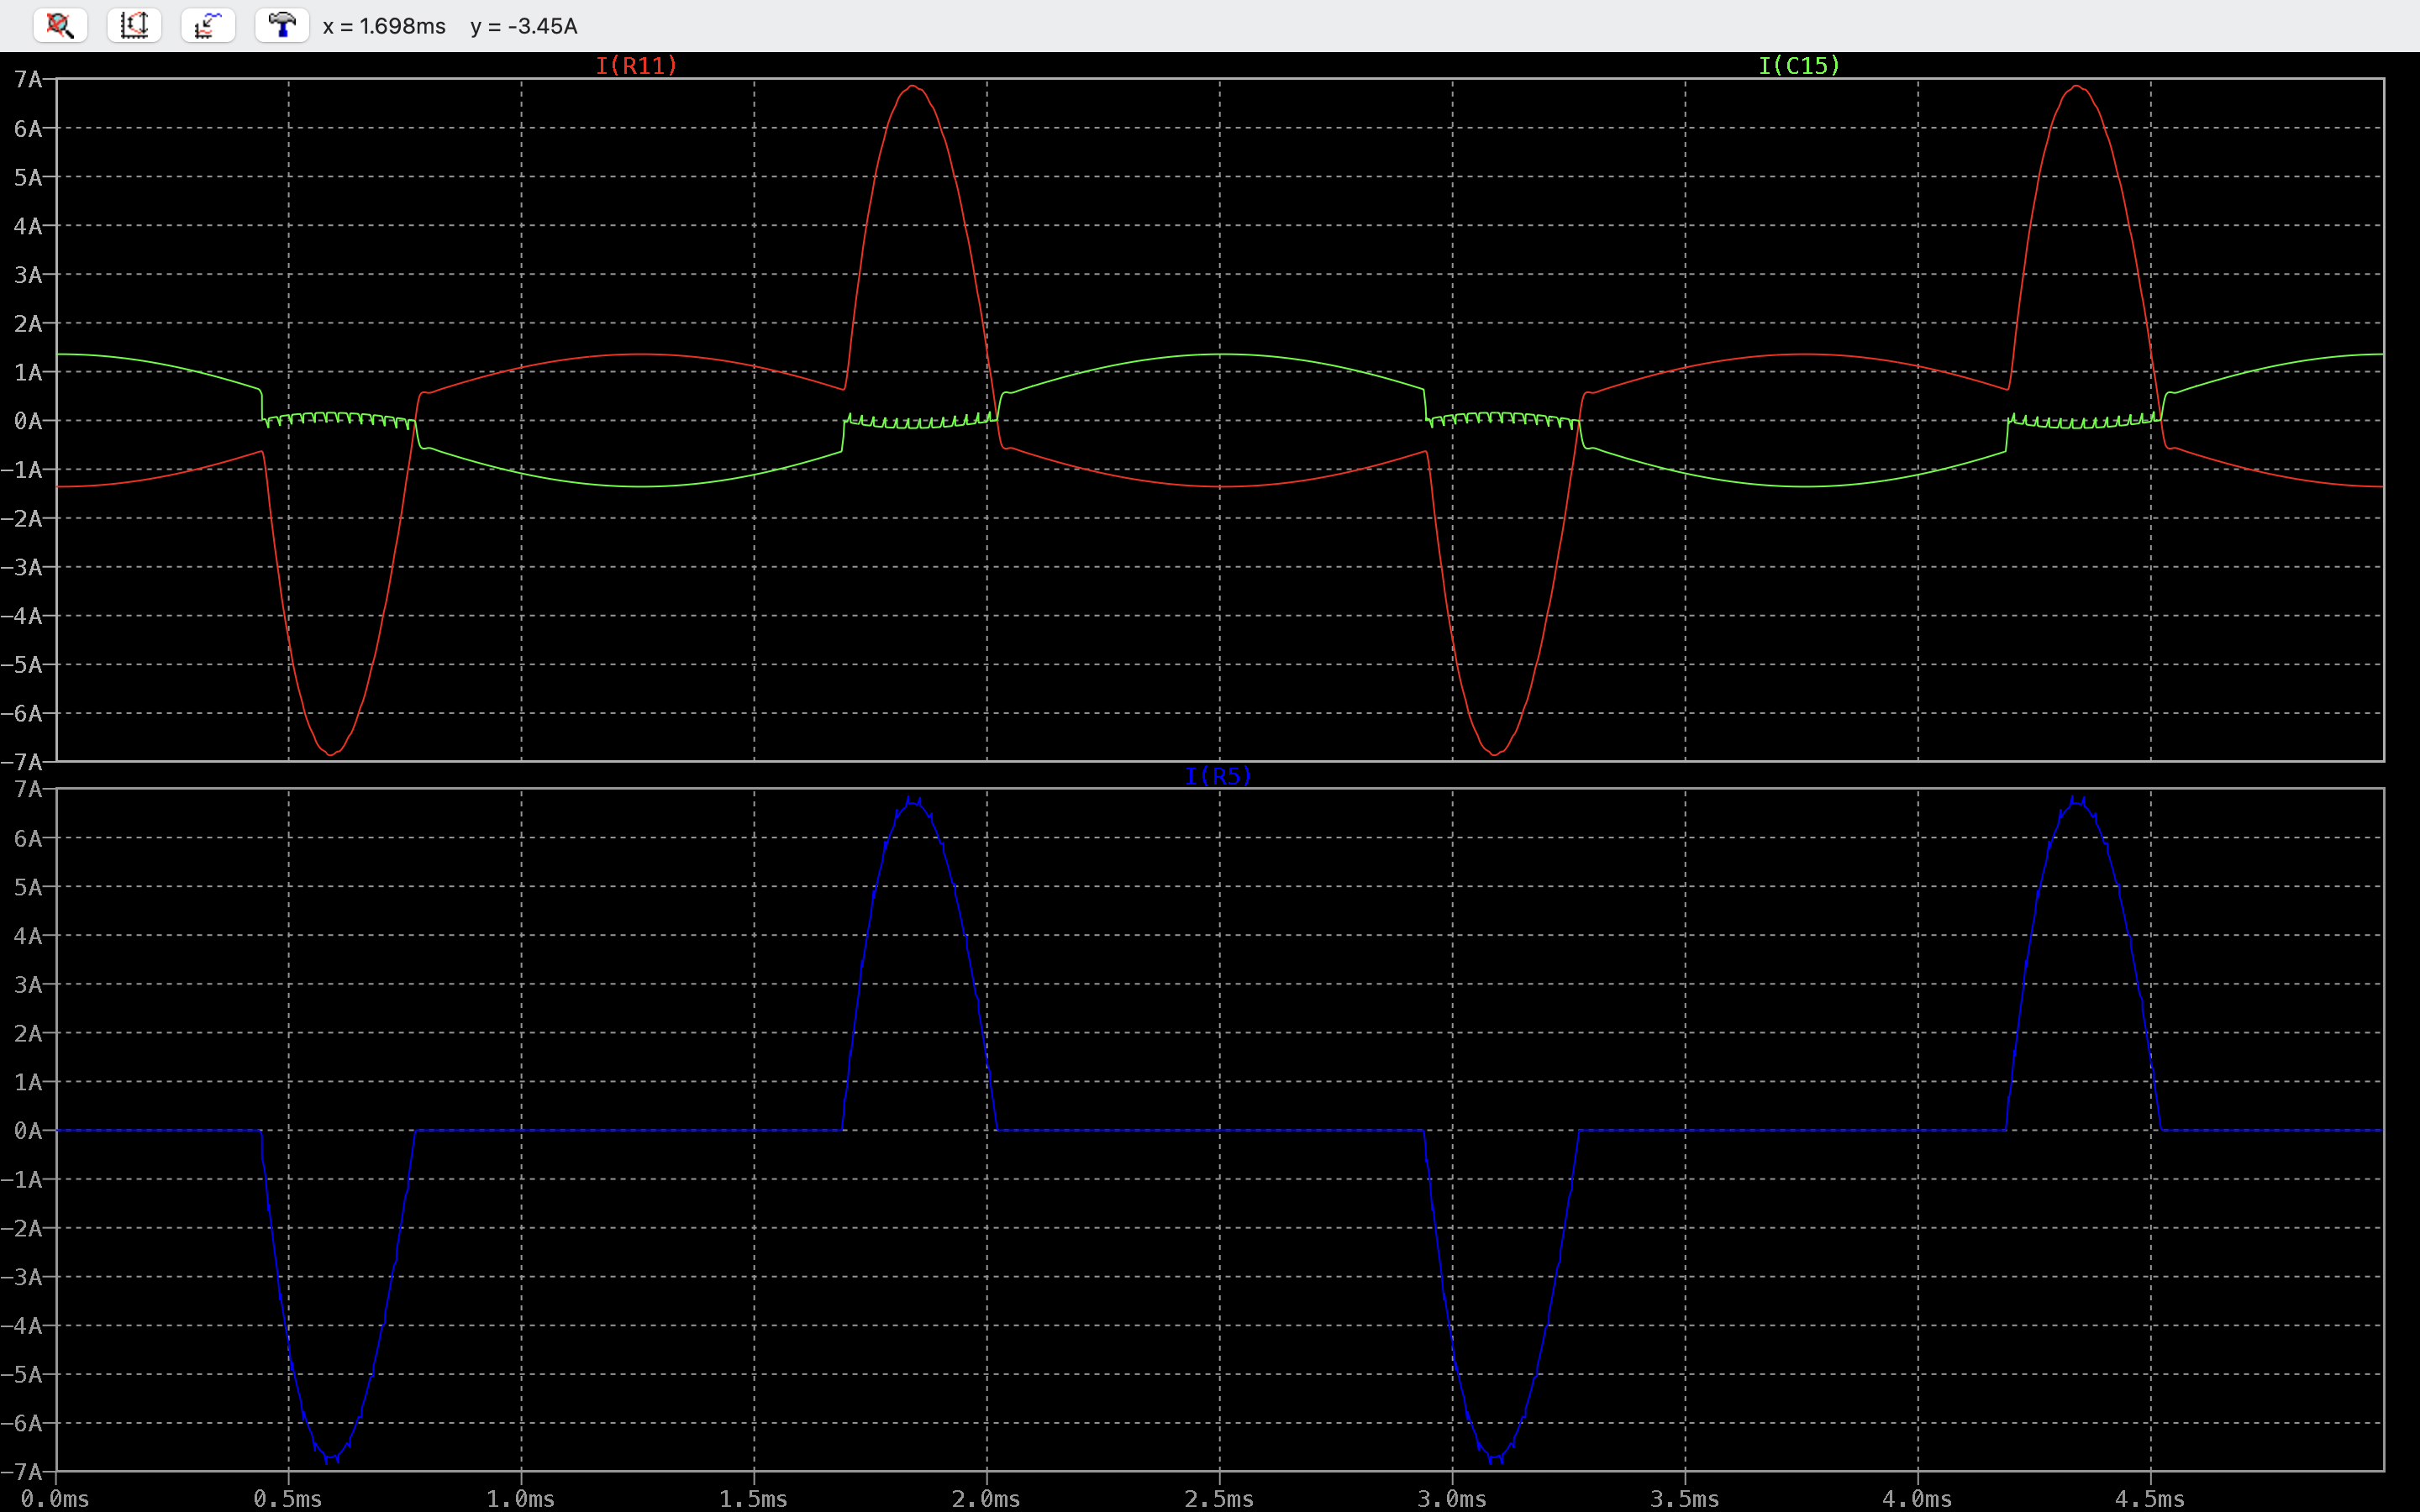
\includegraphics[width=1.0\linewidth]{ac_input_rlc_waveforms.png}
    \caption{RLC Filtering of 115$V_{AC}$ Input}
    \label{fig:ac_input_rlc_waveforms}
\end{figure}

\subsection{Full-Wave Bridge Rectifier}
The full bridge rectifier converts the ac input to a dc output. While the dc output rises, the bulk capacitor $C5$ charges, but when the dc output falls the bulk capacitor discharges. LTSpice simulation shows that the dc output is held stable at around $102V$ but with a voltage ripple of approximately $2.5V$. Figure \ref{fig:full_wave_bridge_rectifier_output_waveform} is a simulation of the voltage output of the full-wave rectifier with bulk capacitance filtering. The bulk capacitor $C5$ is charged by the DC output of the full-wave bridge rectifier

\begin{figure}[htp]
    \centering
    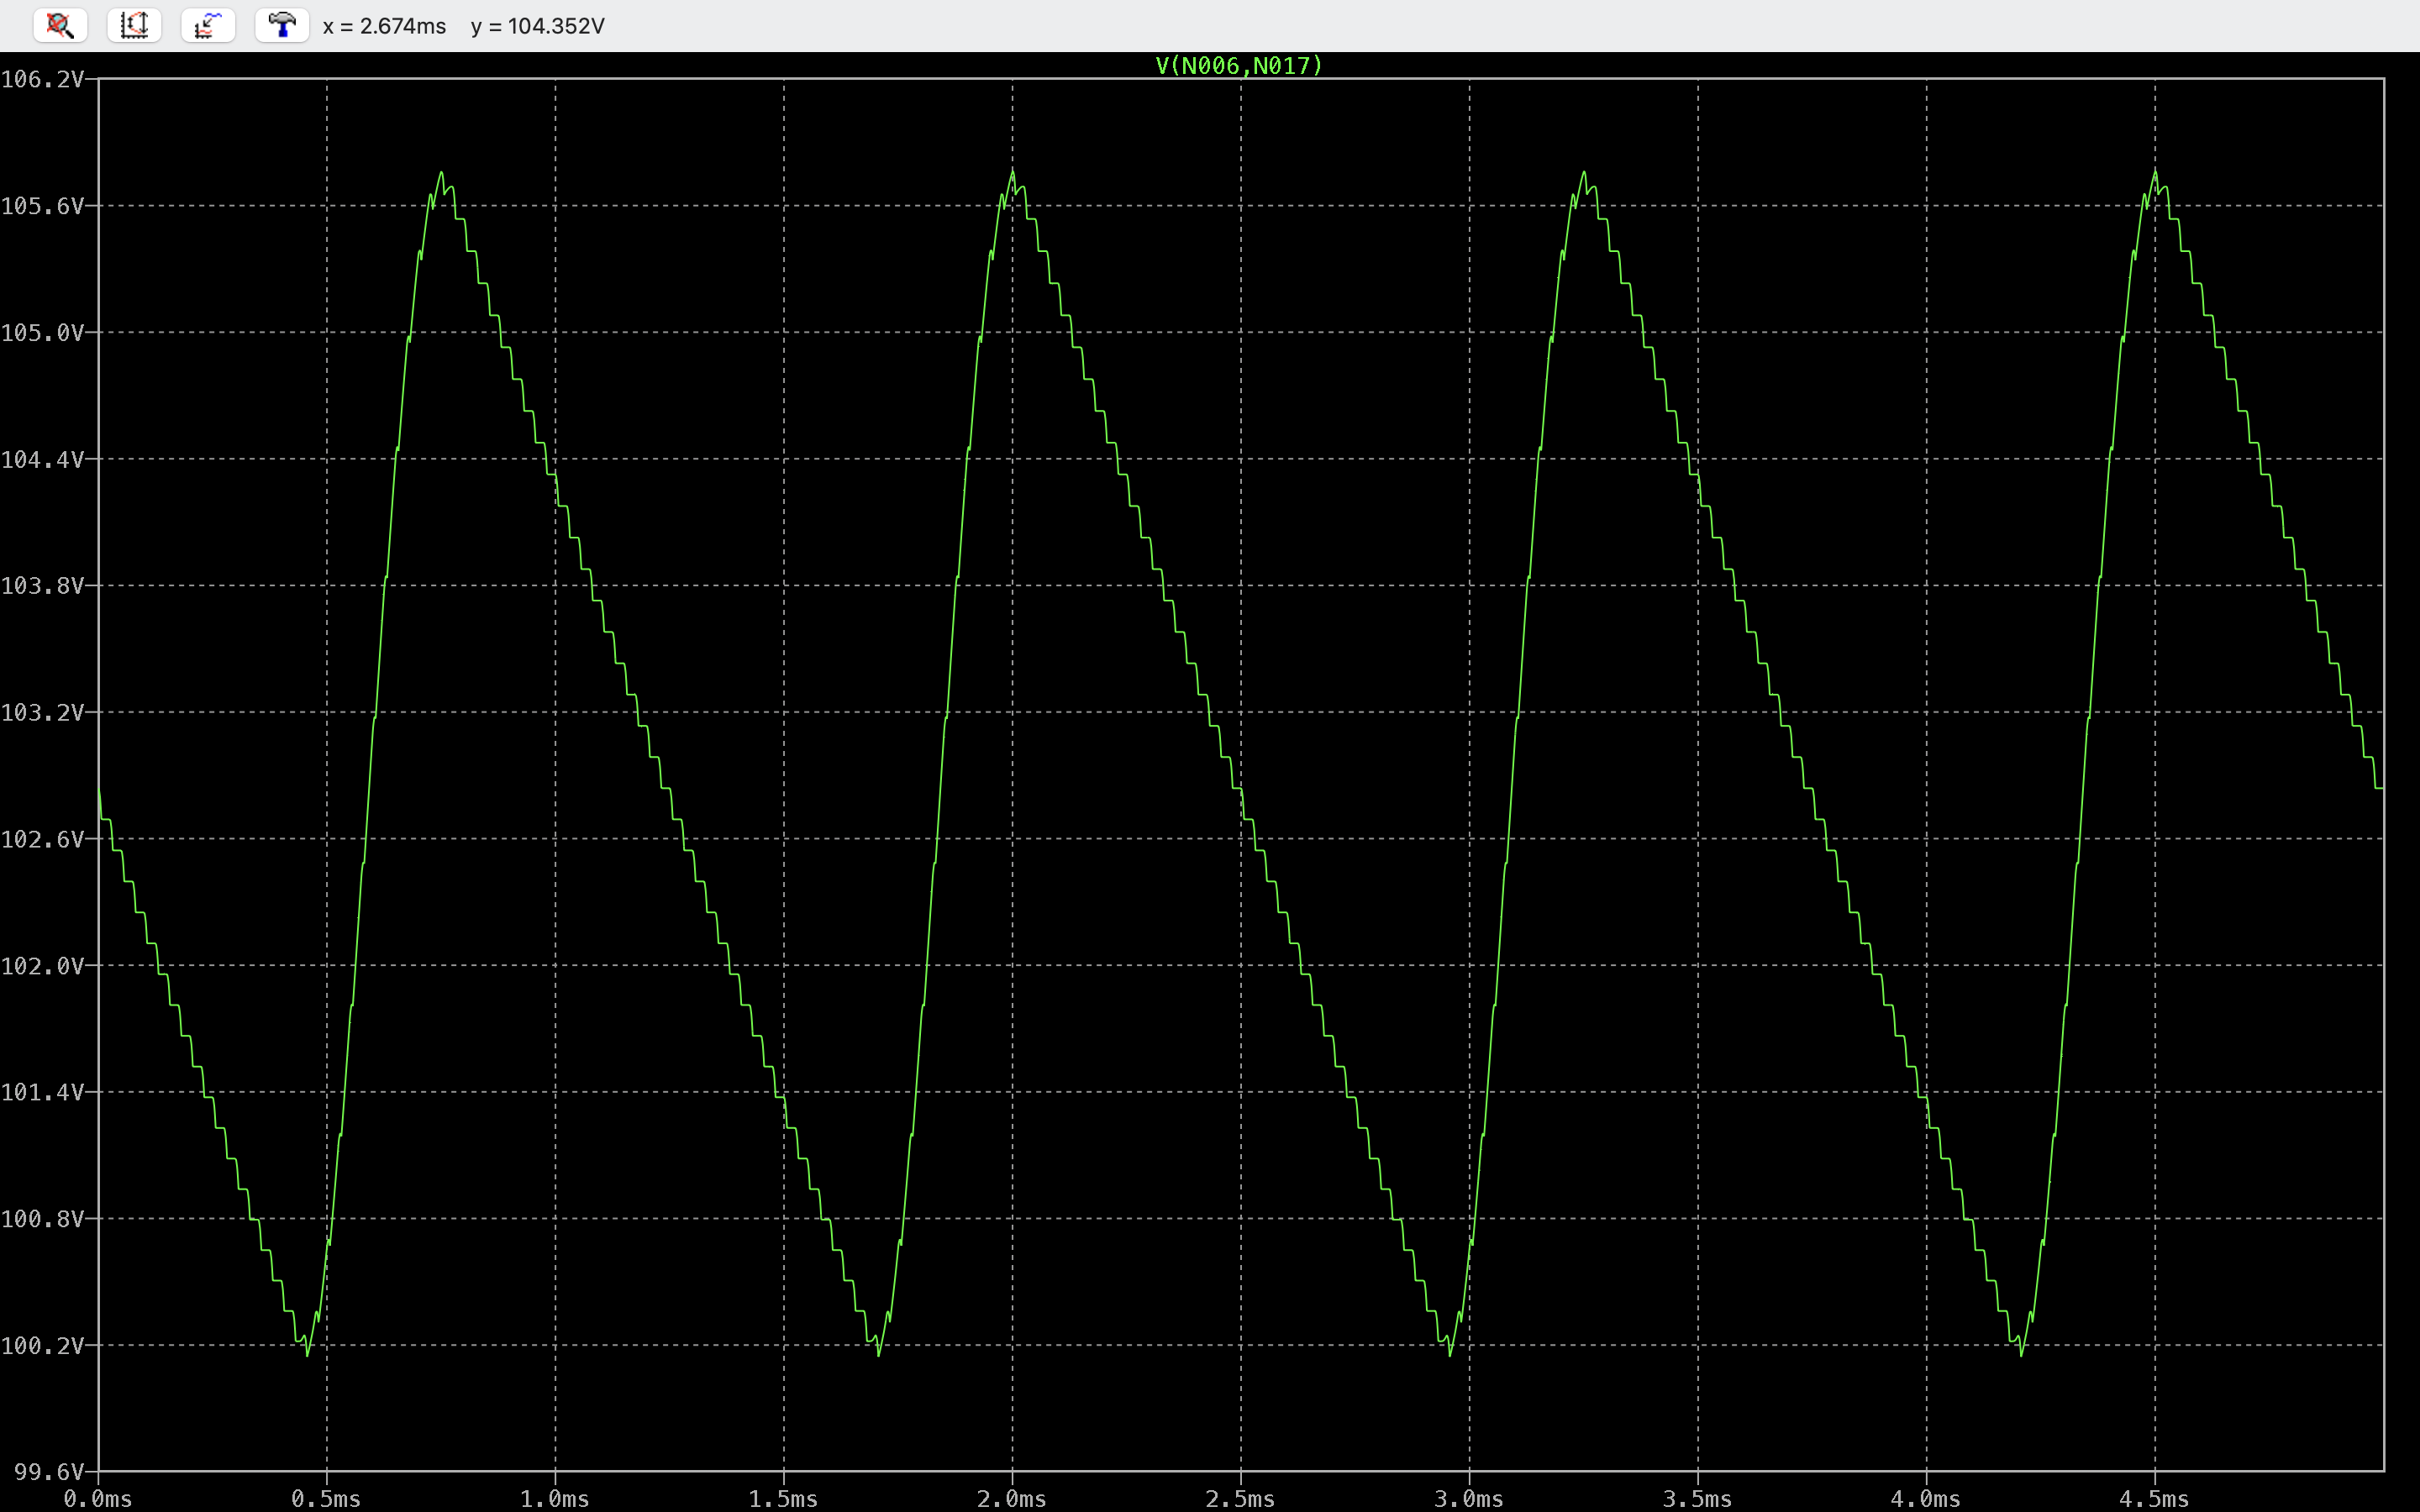
\includegraphics[width=1.0\linewidth]{full_wave_bridge_rectifier_output_waveform.png}
    \caption{Full-Wave Bridge Rectifier Output Voltage}
    \label{fig:full_wave_bridge_rectifier_output_waveform}
\end{figure}

The capacitors $C12$ and $C11$, which connect the power rails to chassis-ground, are included to maintain the relationship of the power rails to ground. In Figure \ref{fig:full_wave_bridge_rectifier_chassis_caps_waveform}, the voltage measured across each capacitor is out-of-phase when compared with the other. The behavior shows that as the bulk capacitor charges, the voltage difference measured across $C12$ increases and the voltage difference measured across $C11$ decreases. Then as the bulk capacitor discharges, the reverse relationship with $C12$ and $C11$ is true.

\begin{figure}[htp]
    \centering
    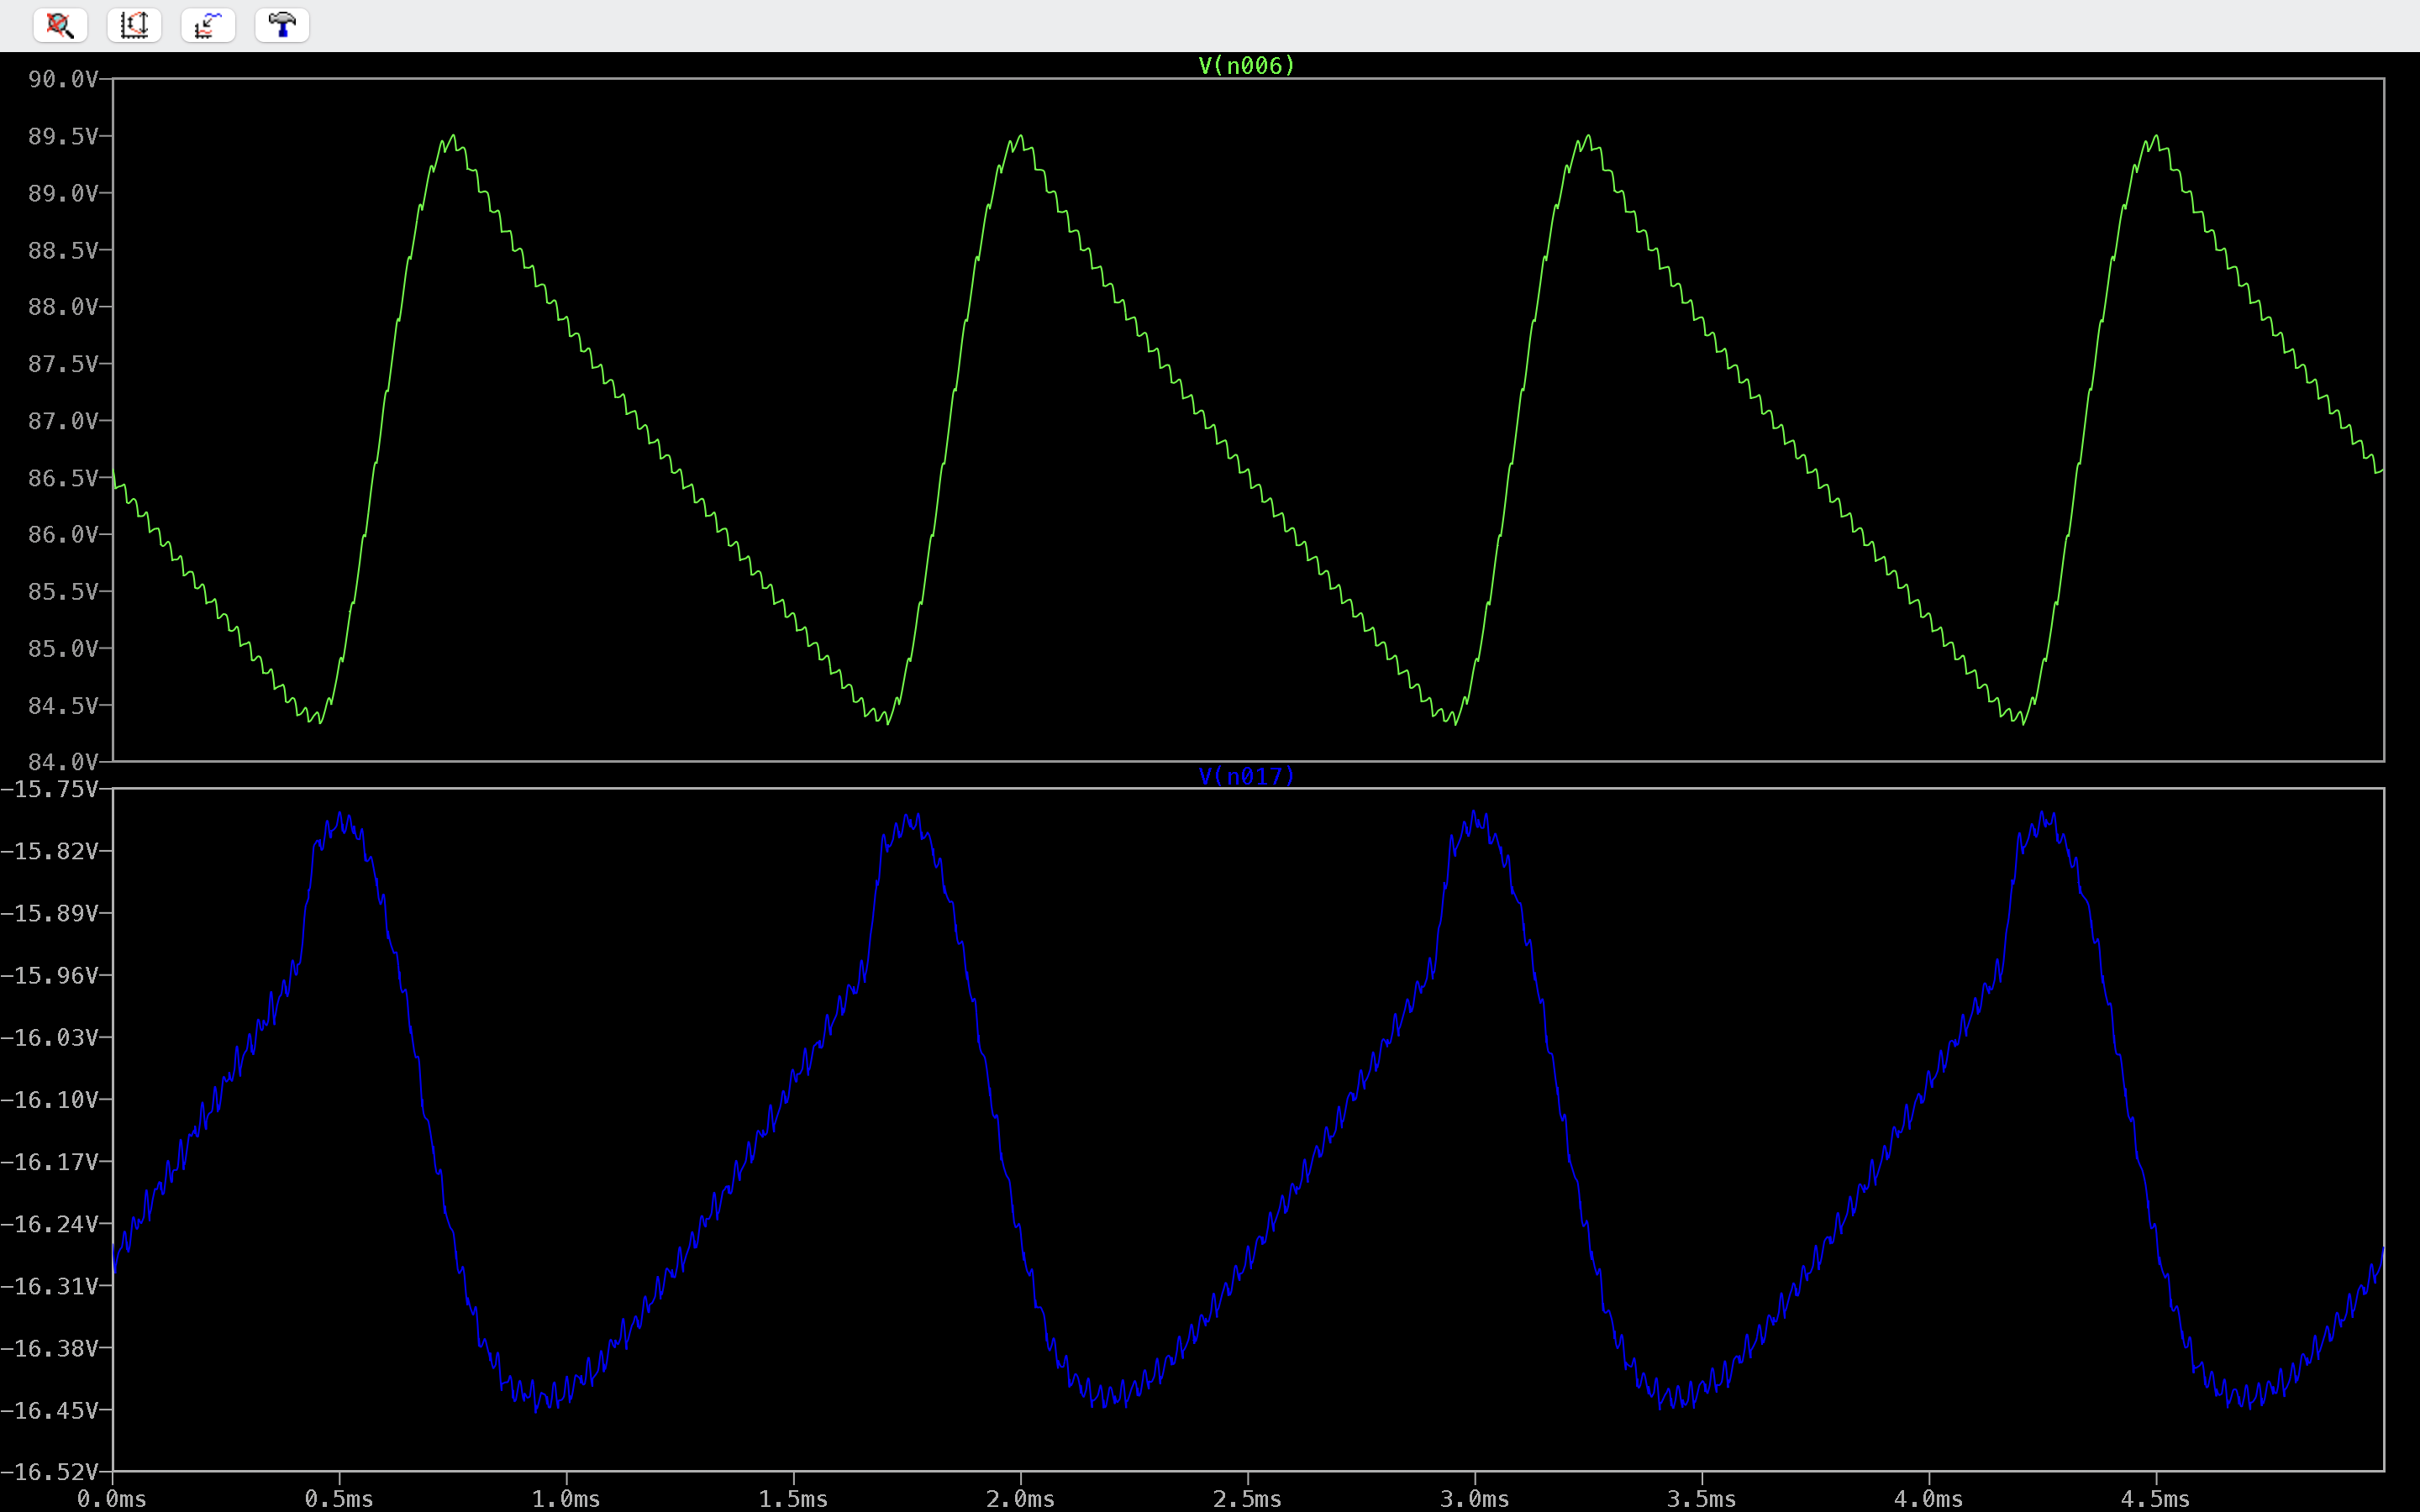
\includegraphics[width=1.0\linewidth]{full_wave_bridge_rectifier_chassis_caps_waveform.png}
    \caption{Voltage across line-to-chassis ground capacitors after Full-Wave Bridge Rectifier}
    \label{fig:full_wave_bridge_rectifier_chassis_caps_waveform}
\end{figure}

\subsection{Buck Converter}

The buck converter drops the full-wave bridge rectifier from 102V to 33.6V as measured across the capacitor $C7$. The current output of the switching regulator is maintained constant by the inductor, $L1$, as demonstrated in Figure \ref{fig:buck_converter_lc_filter_waveforms}. There is a slight discharge and recharge of the inductor as a result of the recharge and discharge of the bulk capacitor on the output of the full-wave bridge rectifier. As a final leg of the buck converter, high frequency noise is shunted to ground by capacitor $C7$. Most of the high frequency noise comes from the switching regulator, so the capacitor is important for immediately removing noise introduced by the switch.

\begin{figure}[htp]
    \centering
    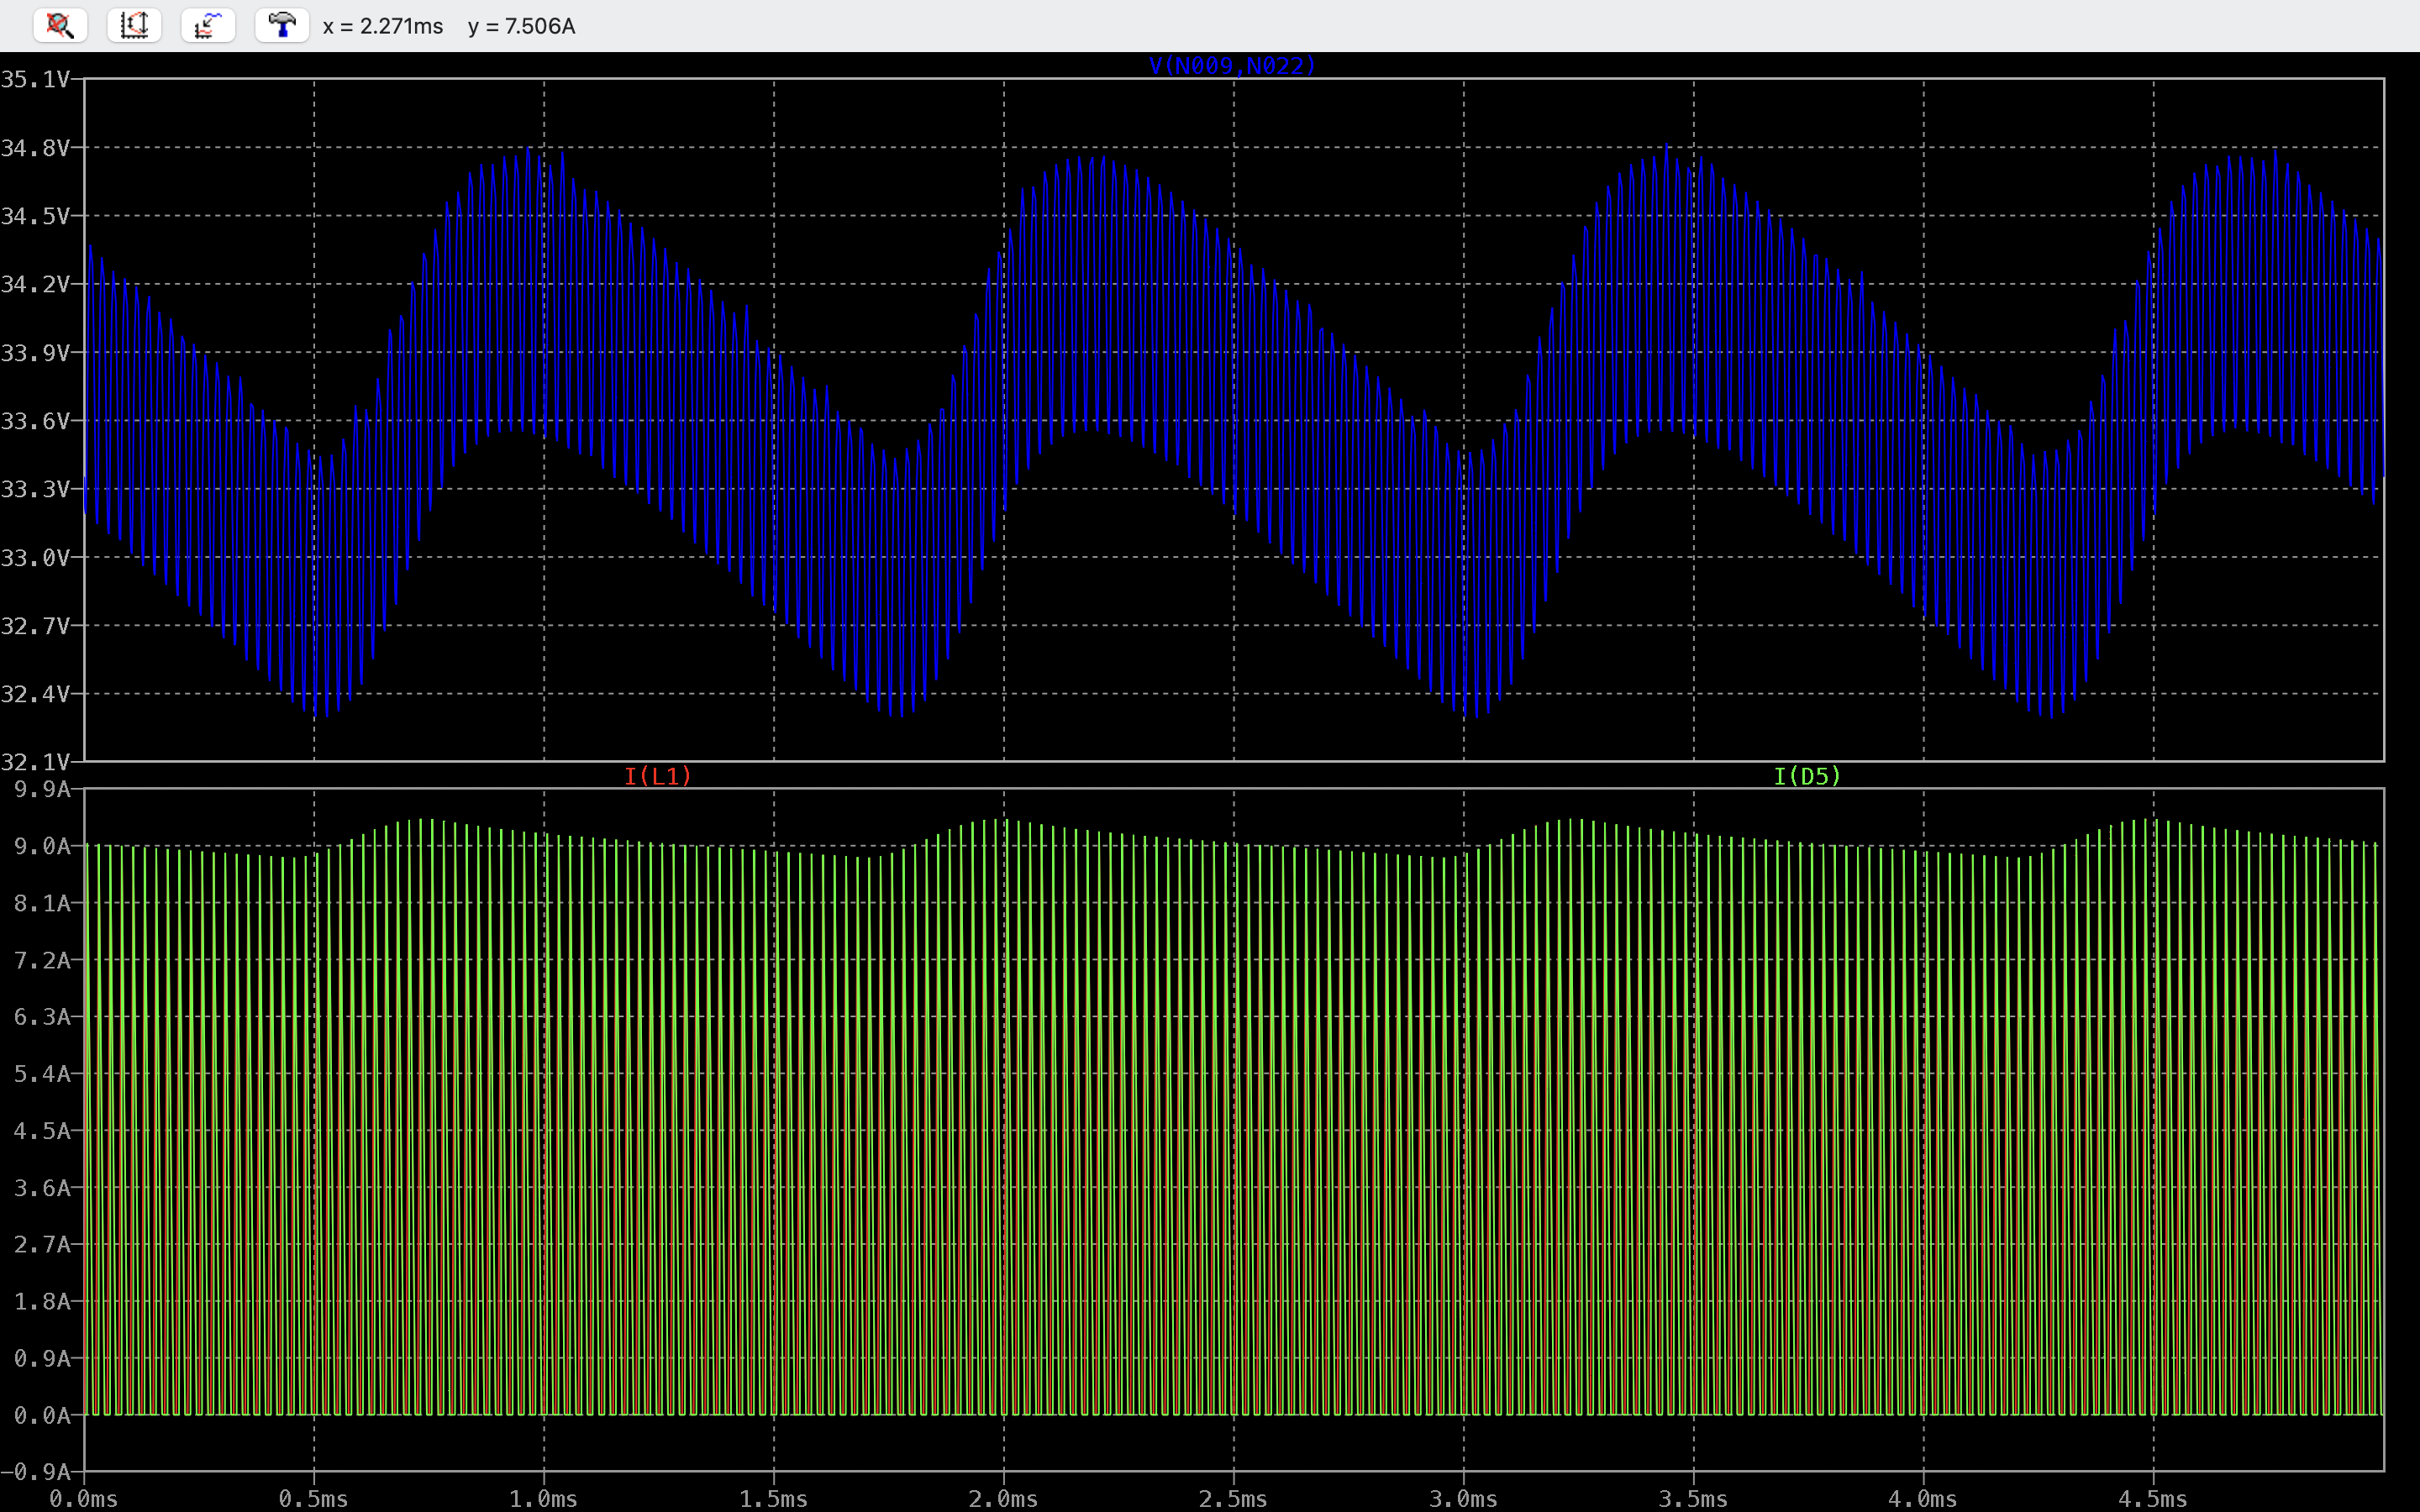
\includegraphics[width=1.0\linewidth]{buck_converter_lc_filter_waveforms.png}
    \caption{Buck Converter Voltage Output}
    \label{fig:buck_converter_lc_filter_waveforms}
\end{figure}

\subsection{Output Filter}
In Figure \ref{fig:output_filter_rlc_stage_1_waveforms} the input voltage of the buck converter is provided and is plotted against the output voltage of the first stage RLC filter, measured across $C7$. There is a slight voltage drop because of $R4$, but more importantly, much of the high-frequency voltage noise from the switch is choked by $L2$. The voltage noise is visibly lower for the $C7$ measurement compared to the $C8$ measurement. The capacitor $C7$ removed much of the high frequency noise on current line, as demonstrated by the current noise seen on the $L2$ current measurement versus the $L5$ current measurement. The power penalty of including the damping resistor $R4$ is about 6.2$W$.

\begin{figure}[htp]
    \centering
    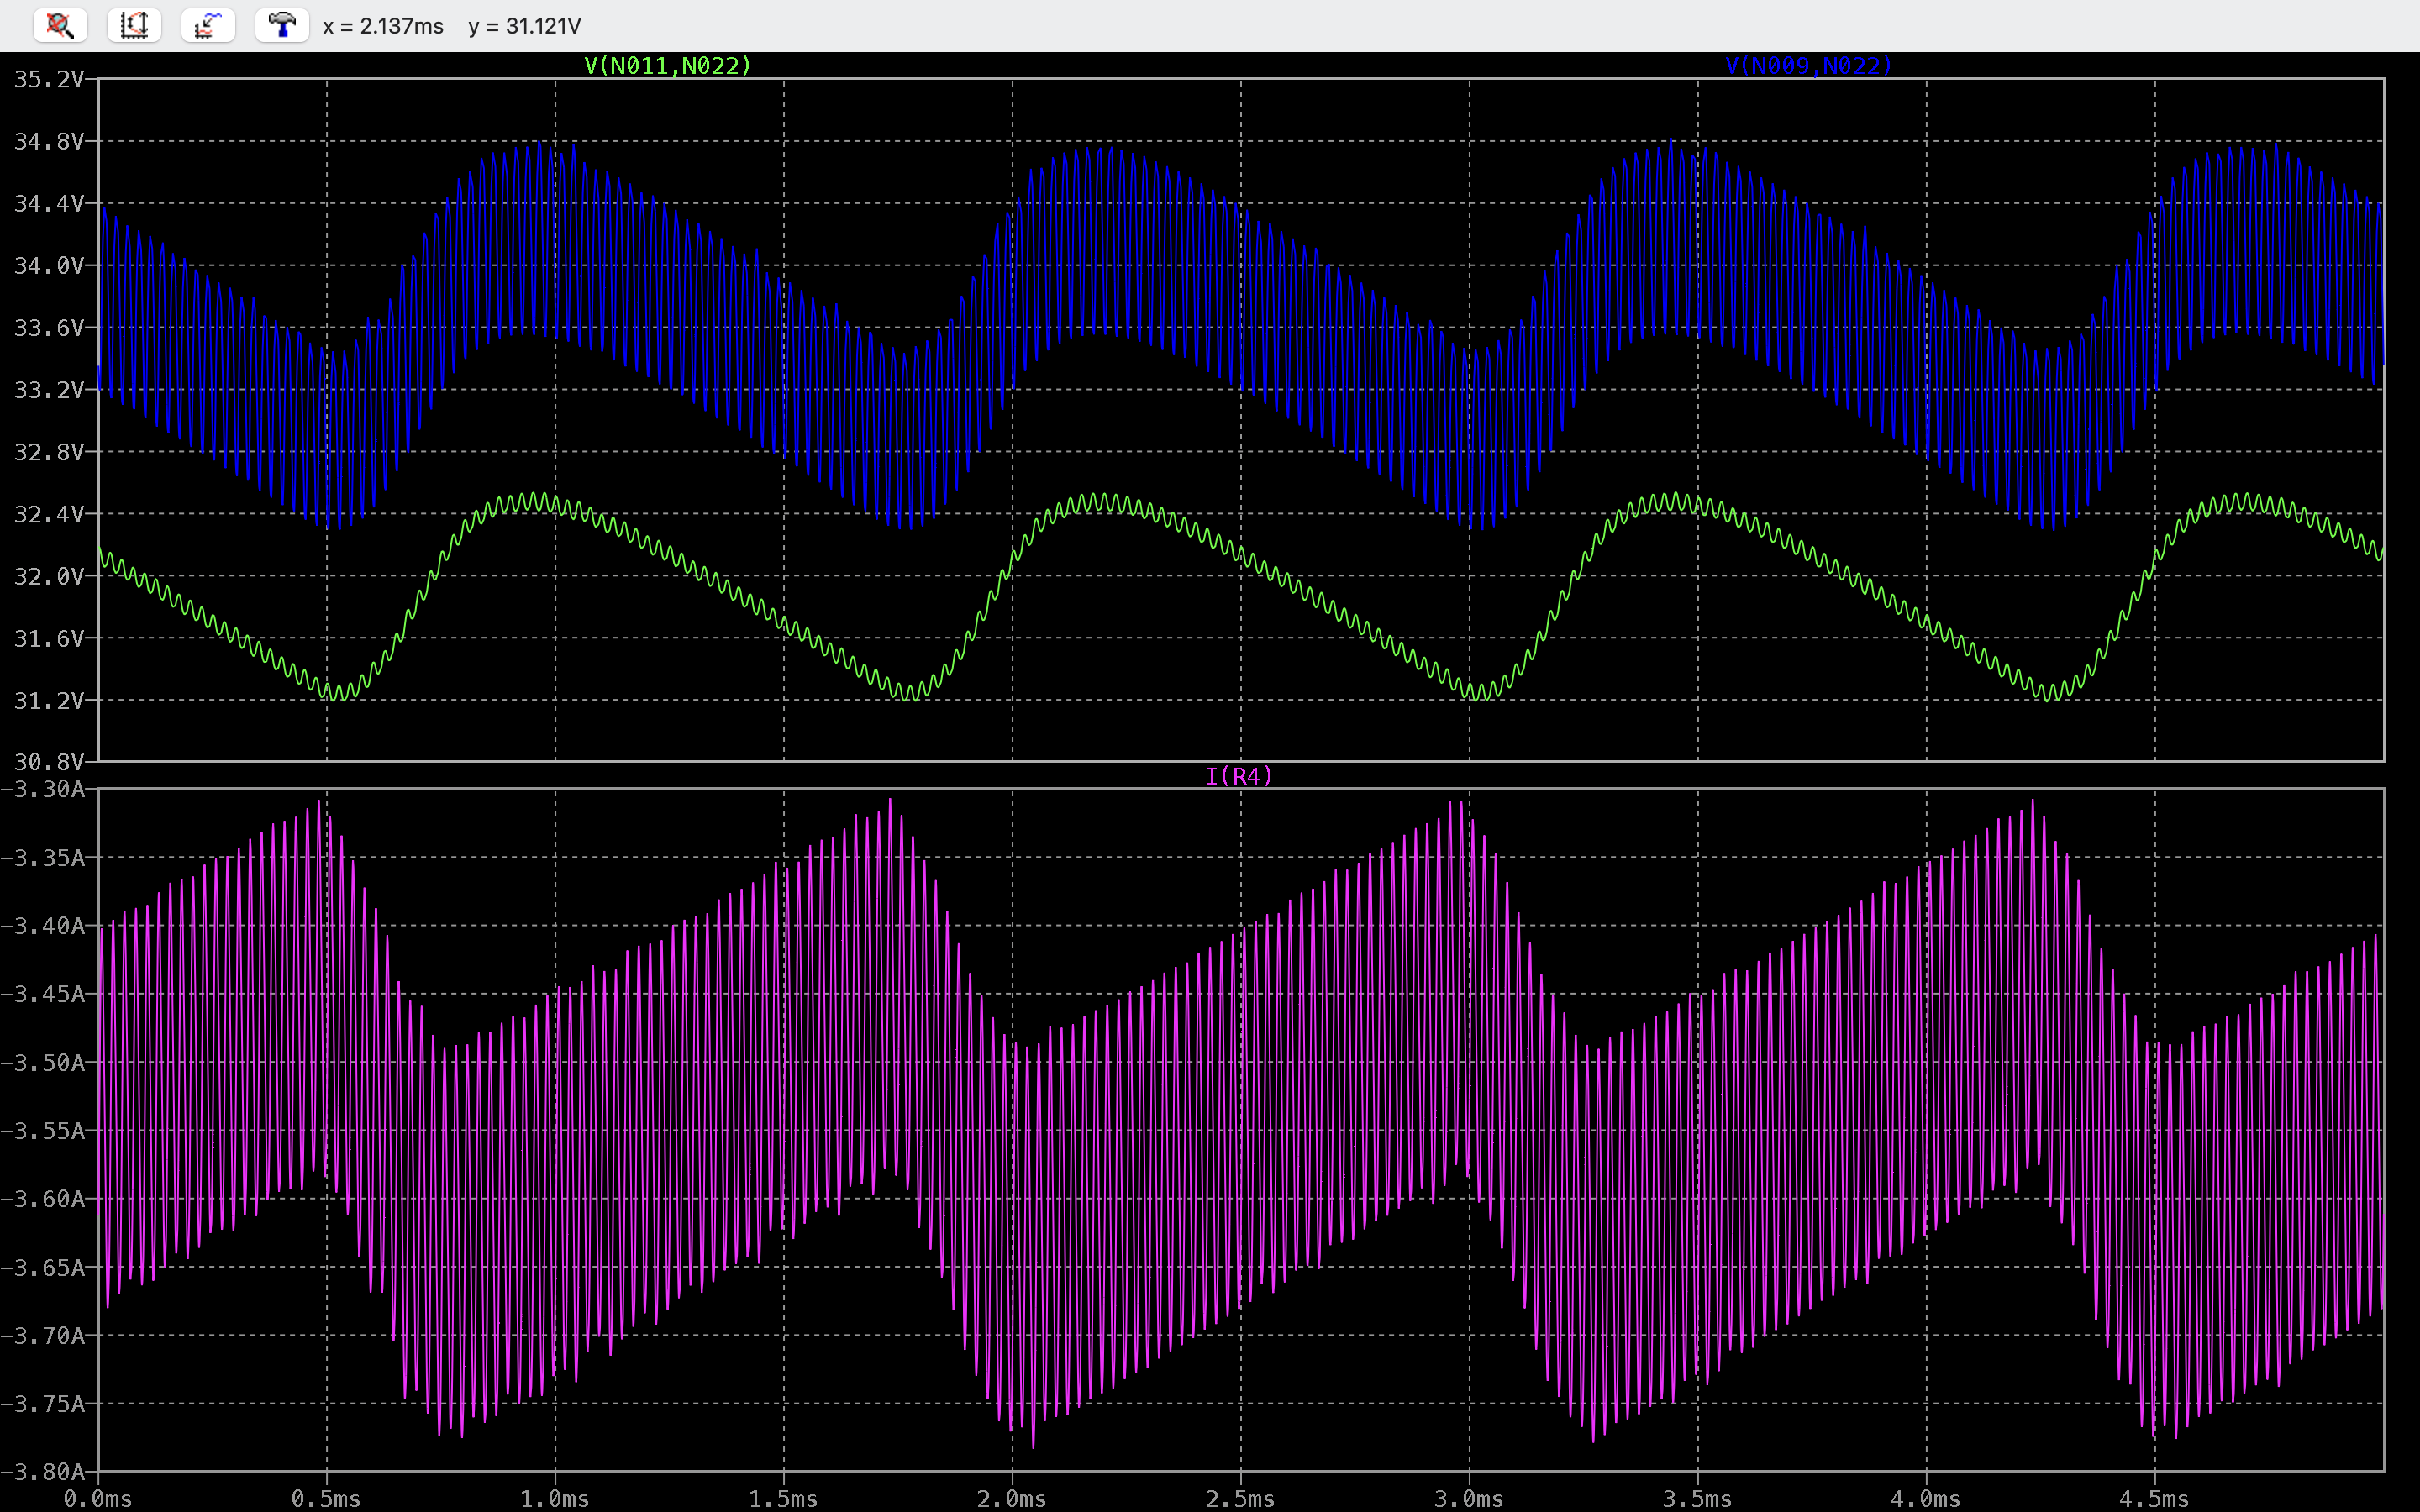
\includegraphics[width=1.0\linewidth]{output_filter_rlc_stage_1.png}
    \caption{Output RLC Filter Stage 1}
    \label{fig:output_filter_rlc_stage_1_waveforms}
\end{figure}

Figure \ref{fig:output_filter_rlc_stage_2_waveforms} continues to demonstrate the voltage noise and current noise clean-up that was discussed for the first stage current measurement. The power penalty of including the damping resistor $R3$ is about 12.6$W$

\begin{figure}[htp]
    \centering
    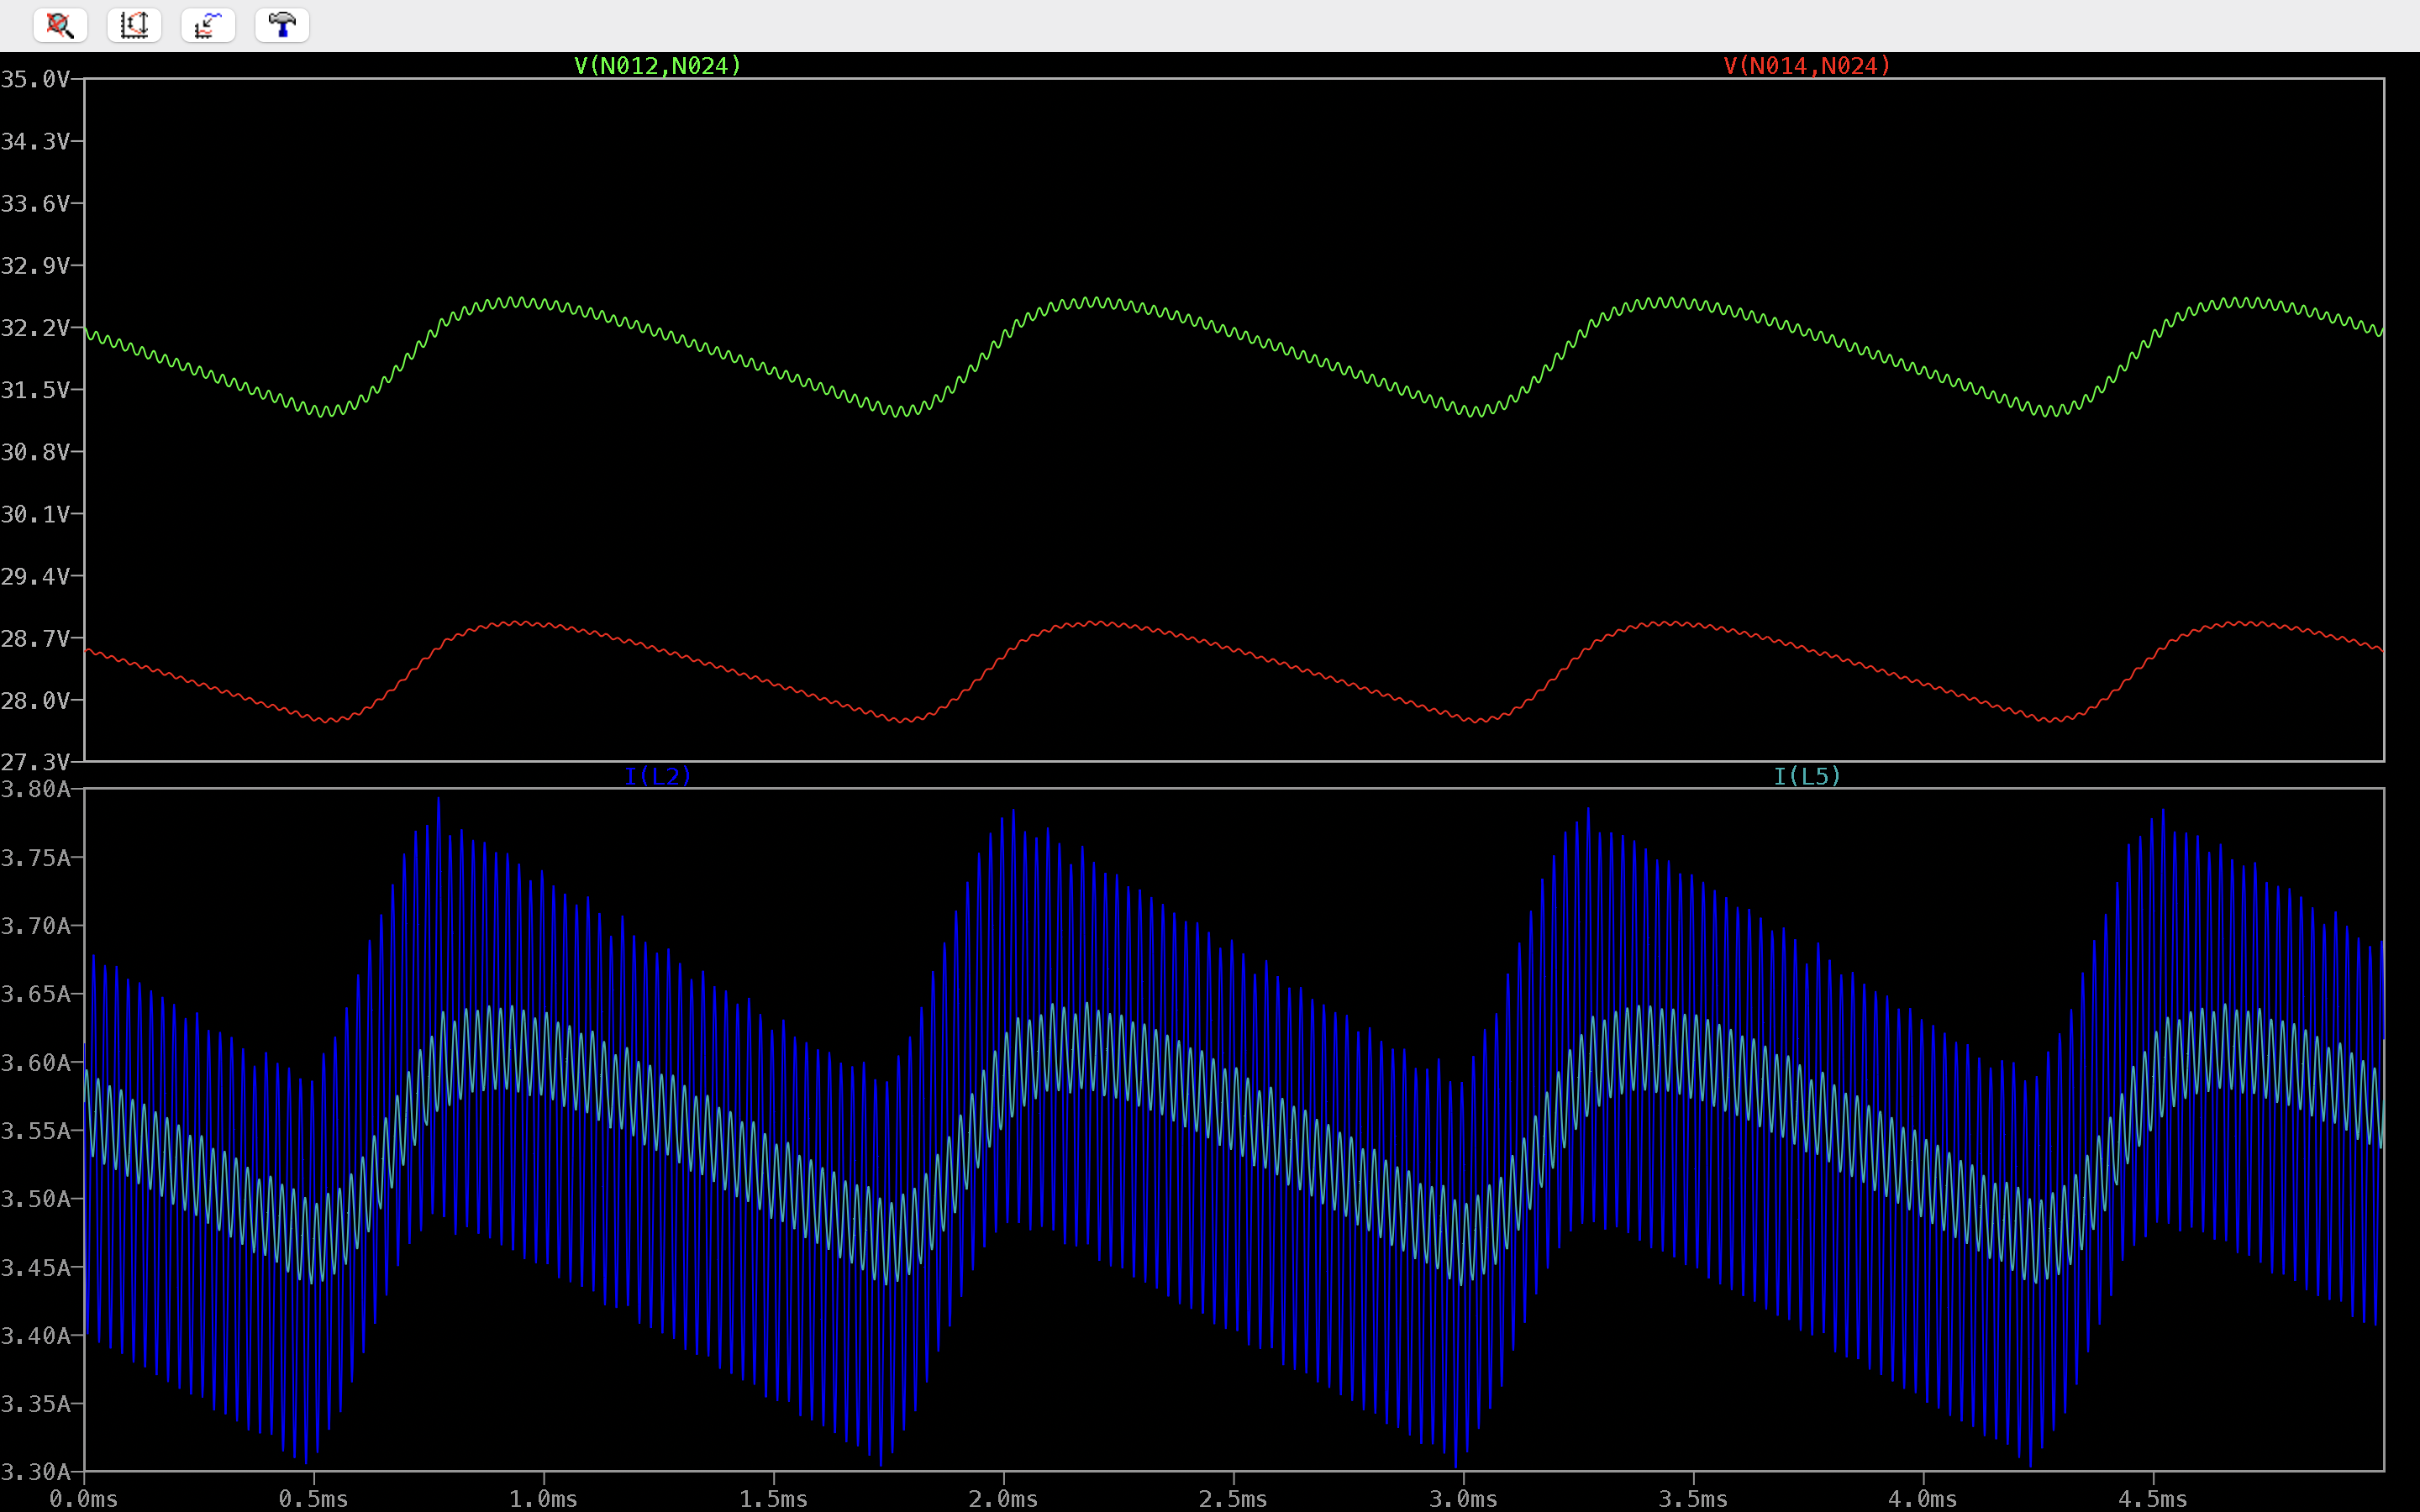
\includegraphics[width=1.0\linewidth]{output_filter_rlc_stage_2.png}
    \caption{Output RLC Filter Stage 2}
    \label{fig:output_filter_rlc_stage_2_waveforms}
\end{figure}

The 

Figure \ref{fig:output_filter_common_mode_choke_waveforms}

\begin{figure}[htp]
    \centering
    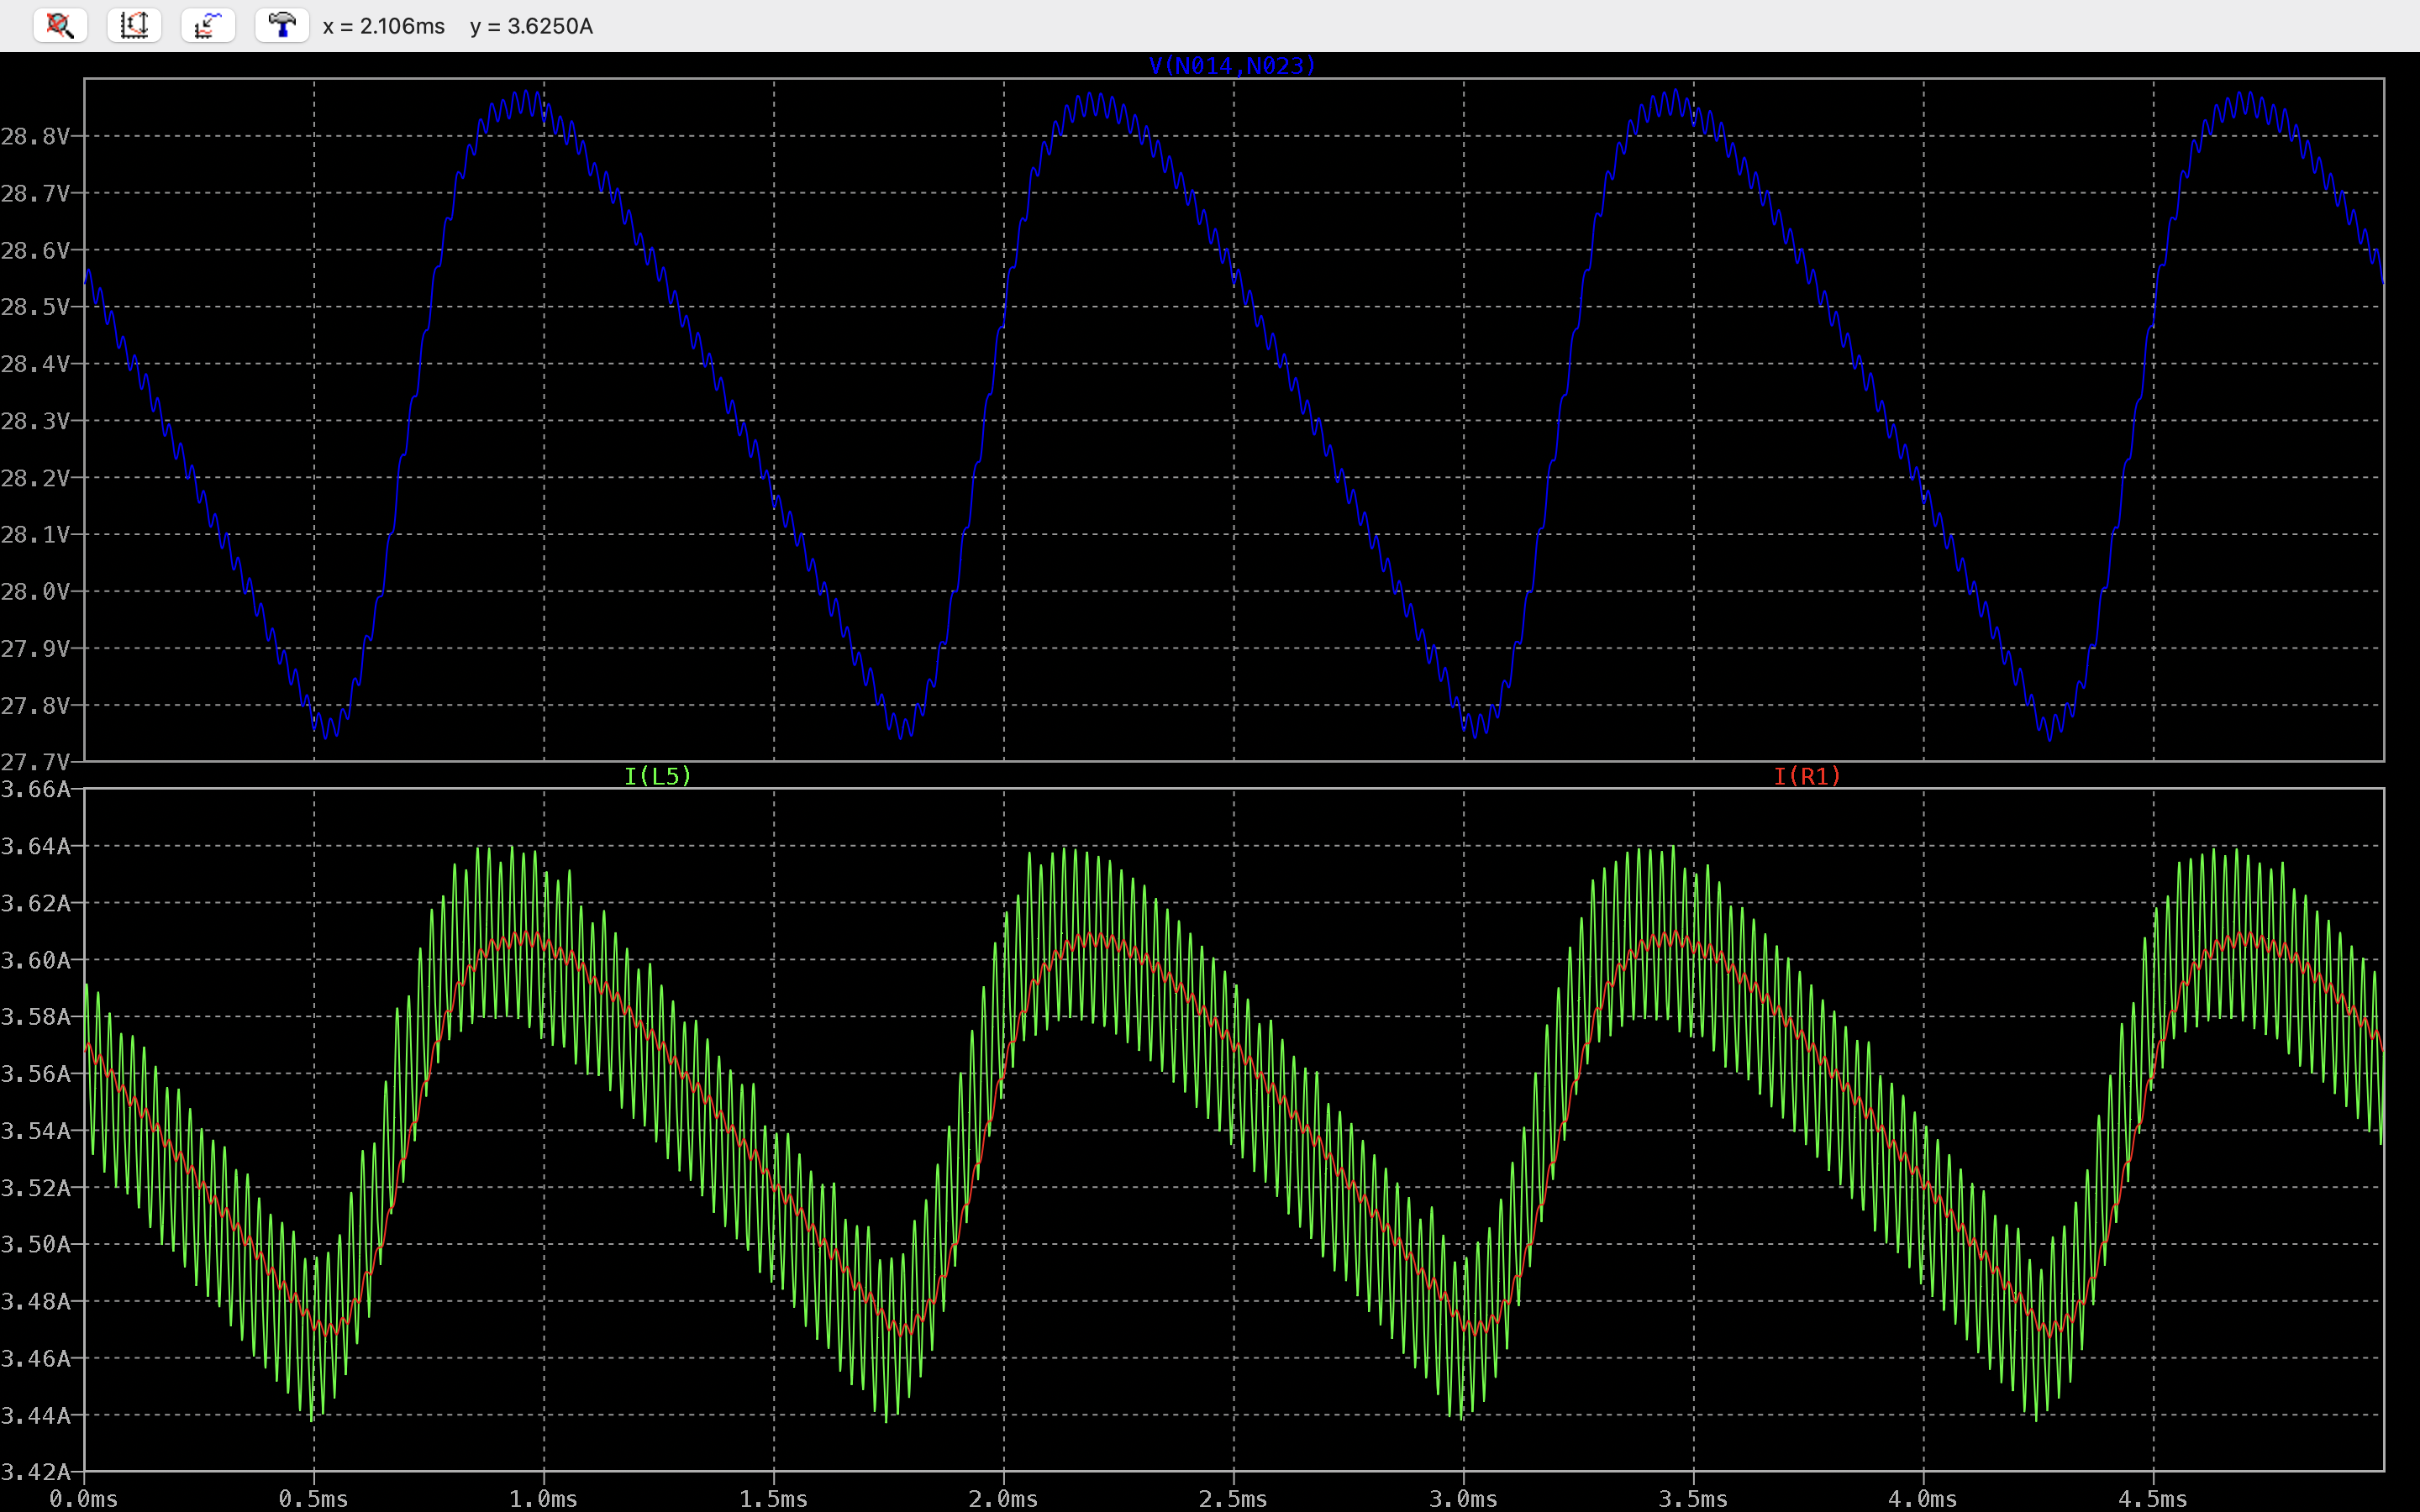
\includegraphics[width=1.0\linewidth]{output_filter_common_mode_choke.png}
    \caption{Output Filter Common Mode Choke Current}
    \label{fig:output_filter_common_mode_choke_waveforms}
\end{figure}

In addition to the common-mode choke, the noise current across the line to chassis-ground capacitors on the unit side and the load side were very small as seen in Figure \ref{fig:output_filter_chassis_ground_y_capacitors_waveforms}. There was very little common-mode noise risk from either the load side or source side threatening the AC-DC converter circuit.  

\begin{figure}[htp]
    \centering
    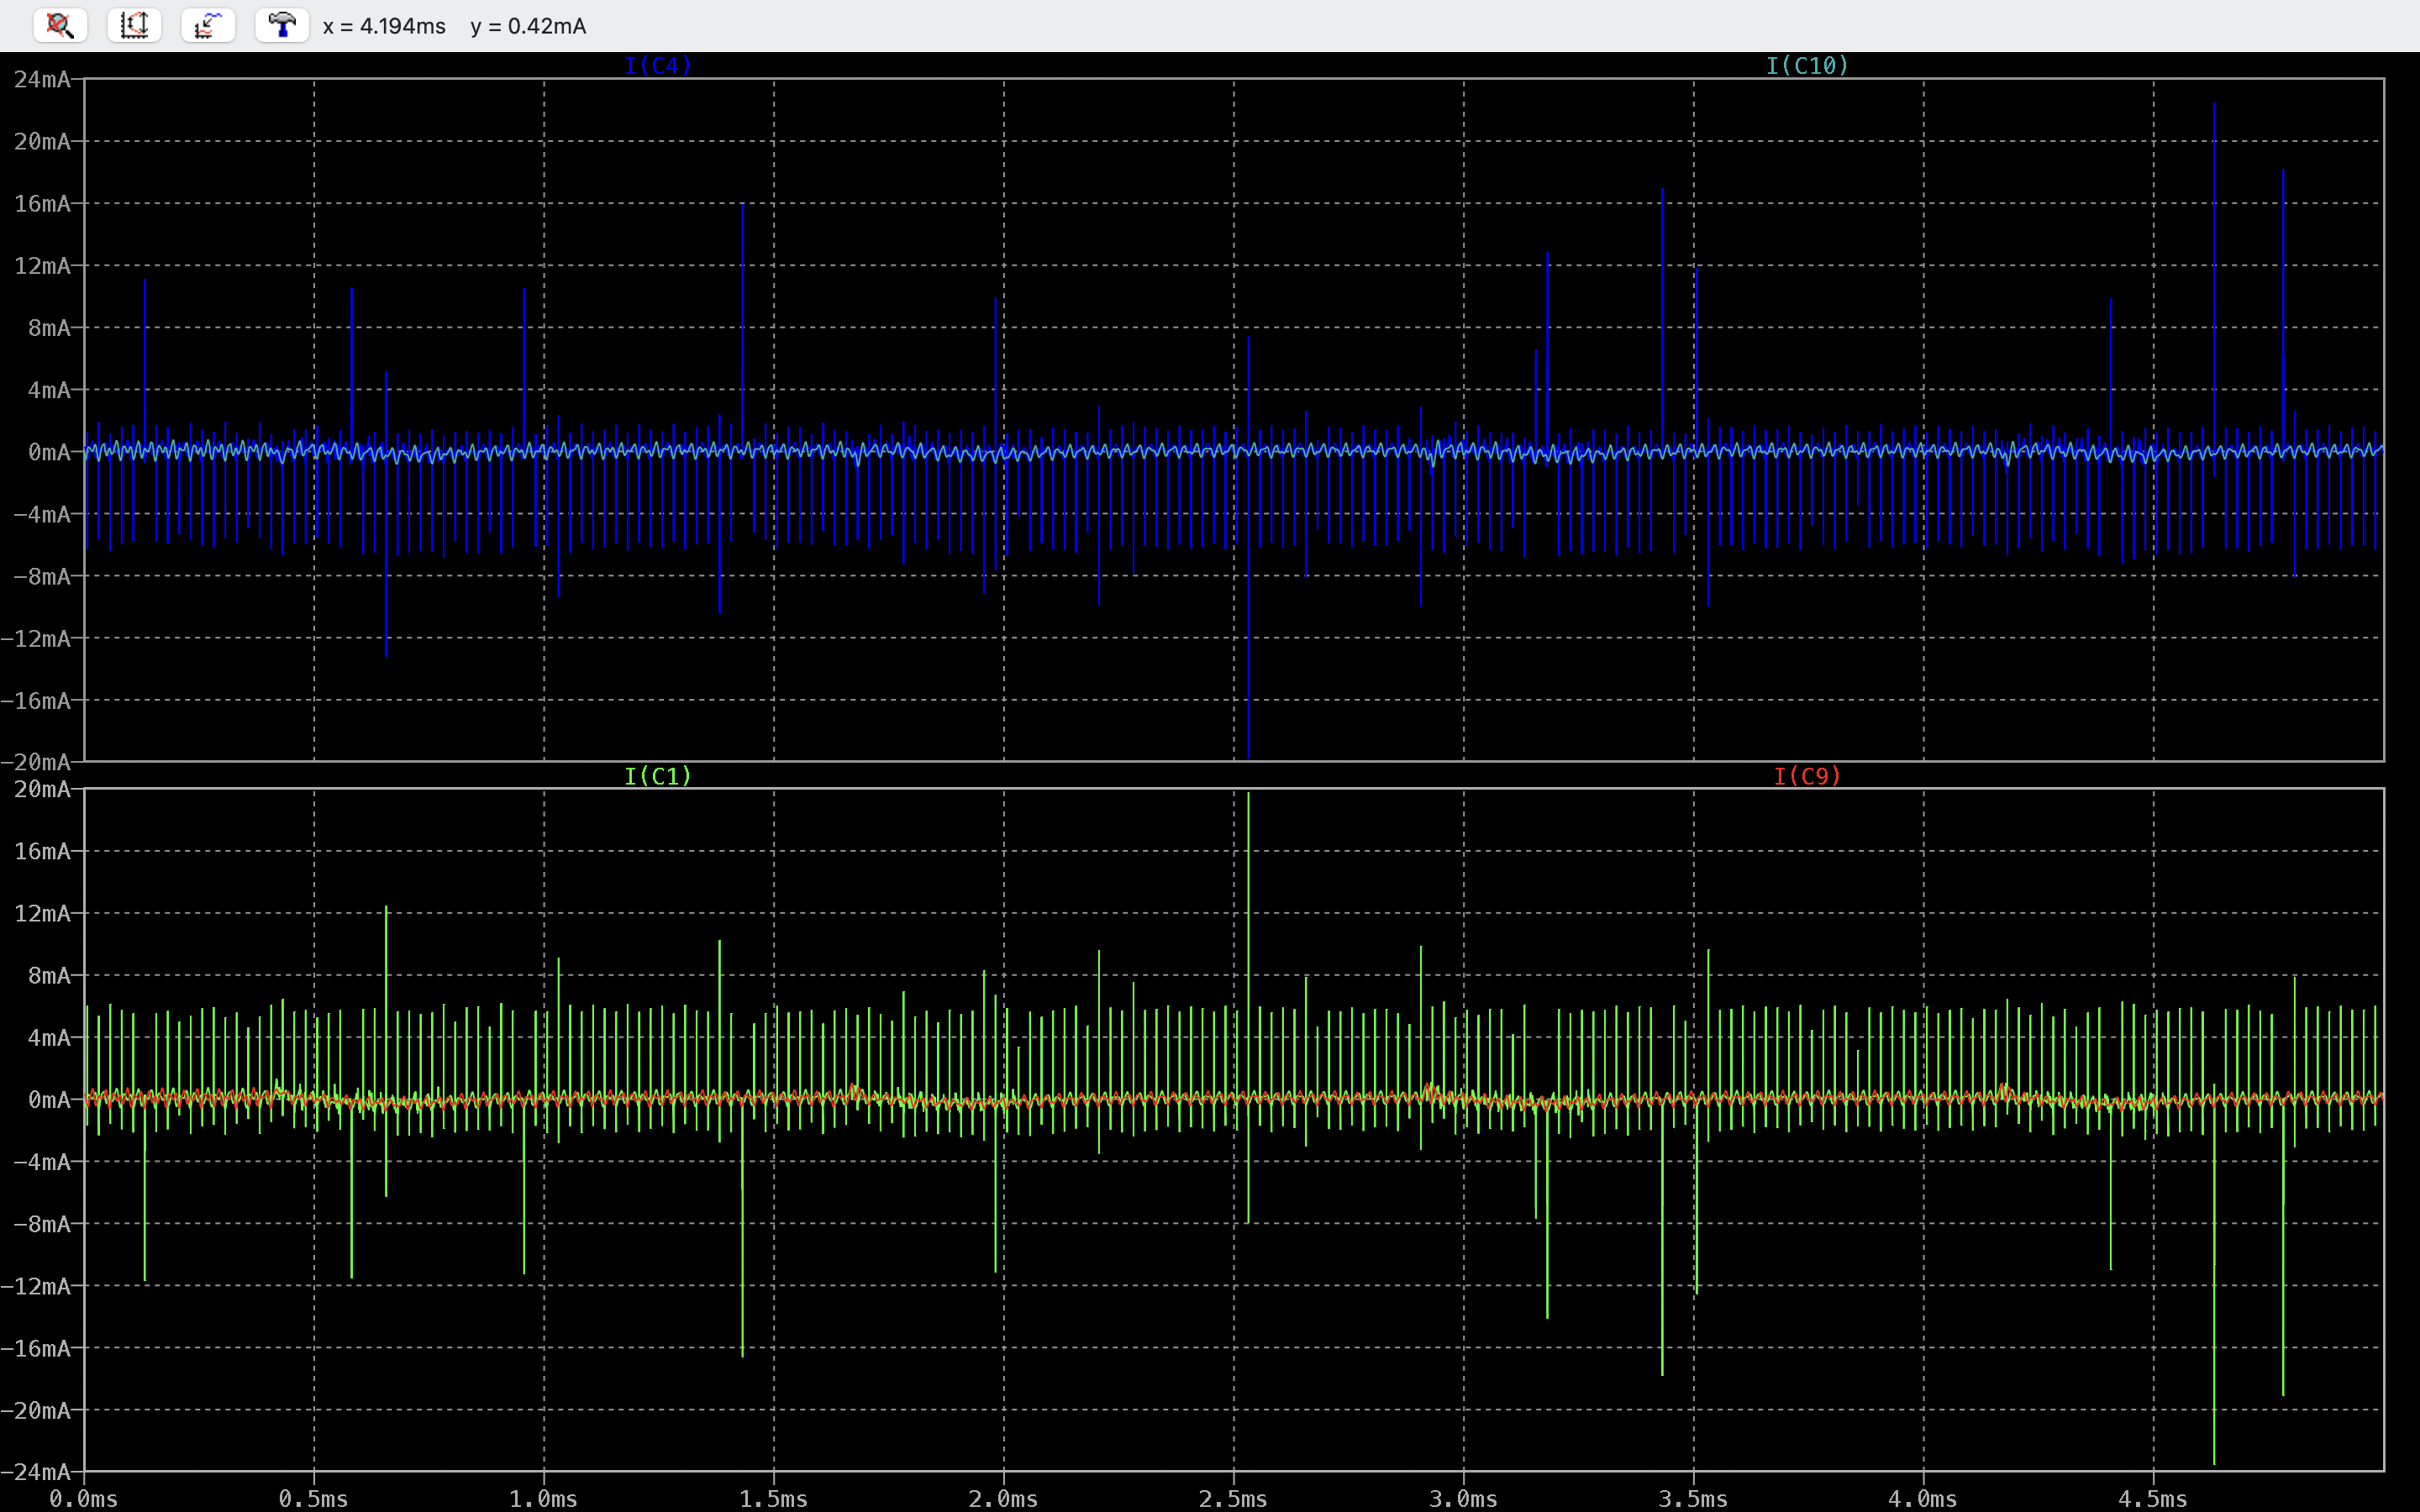
\includegraphics[width=1.0\linewidth]{output_filter_chassis_ground_y_capacitors.png}
    \caption{Current across line-to-chassis ground Y-Capacitor}
    \label{fig:output_filter_chassis_ground_y_capacitors_waveforms}
\end{figure}

\subsection{Load}

Figure \ref{fig:load_average_voltage_waveform}
Figure \ref{fig:load_fft_150kHz_16MHz_waveform}

\begin{figure}[htp]
    \centering
    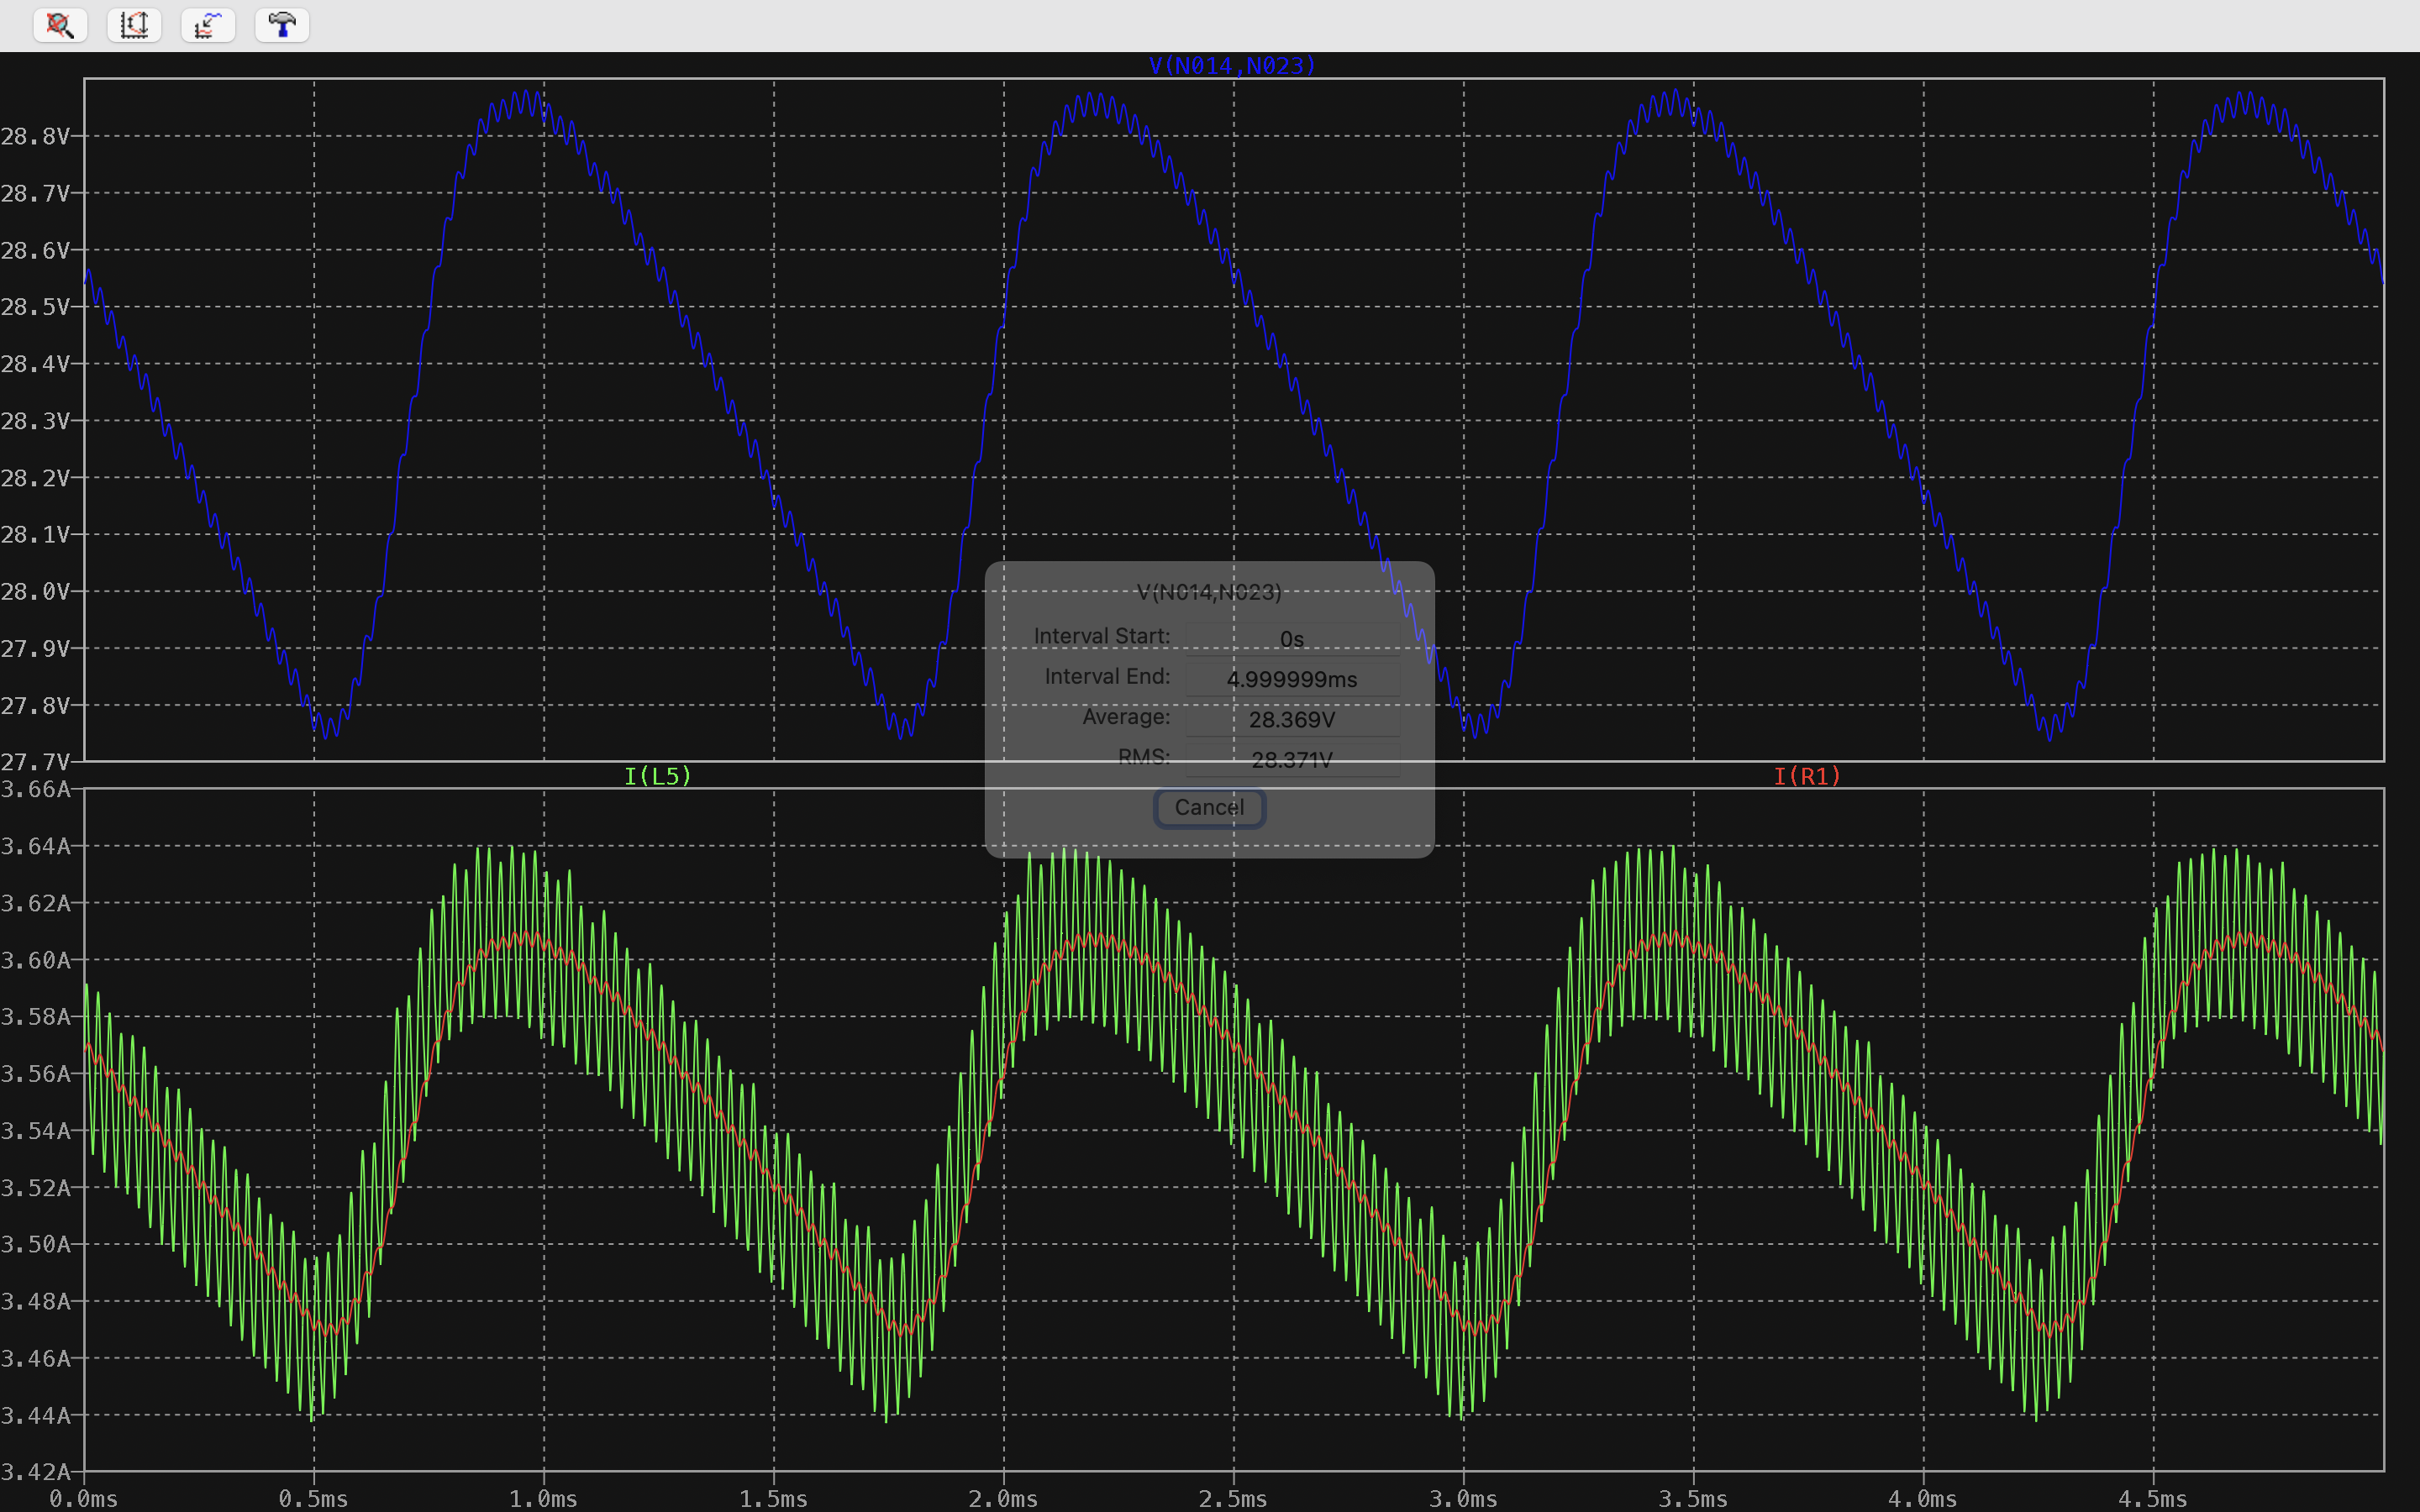
\includegraphics[width=1.0\linewidth]{load_average_voltage.png}
    \caption{Average voltage across load}
    \label{fig:load_average_voltage_waveform}
\end{figure}

\begin{figure}[htp]
    \centering
    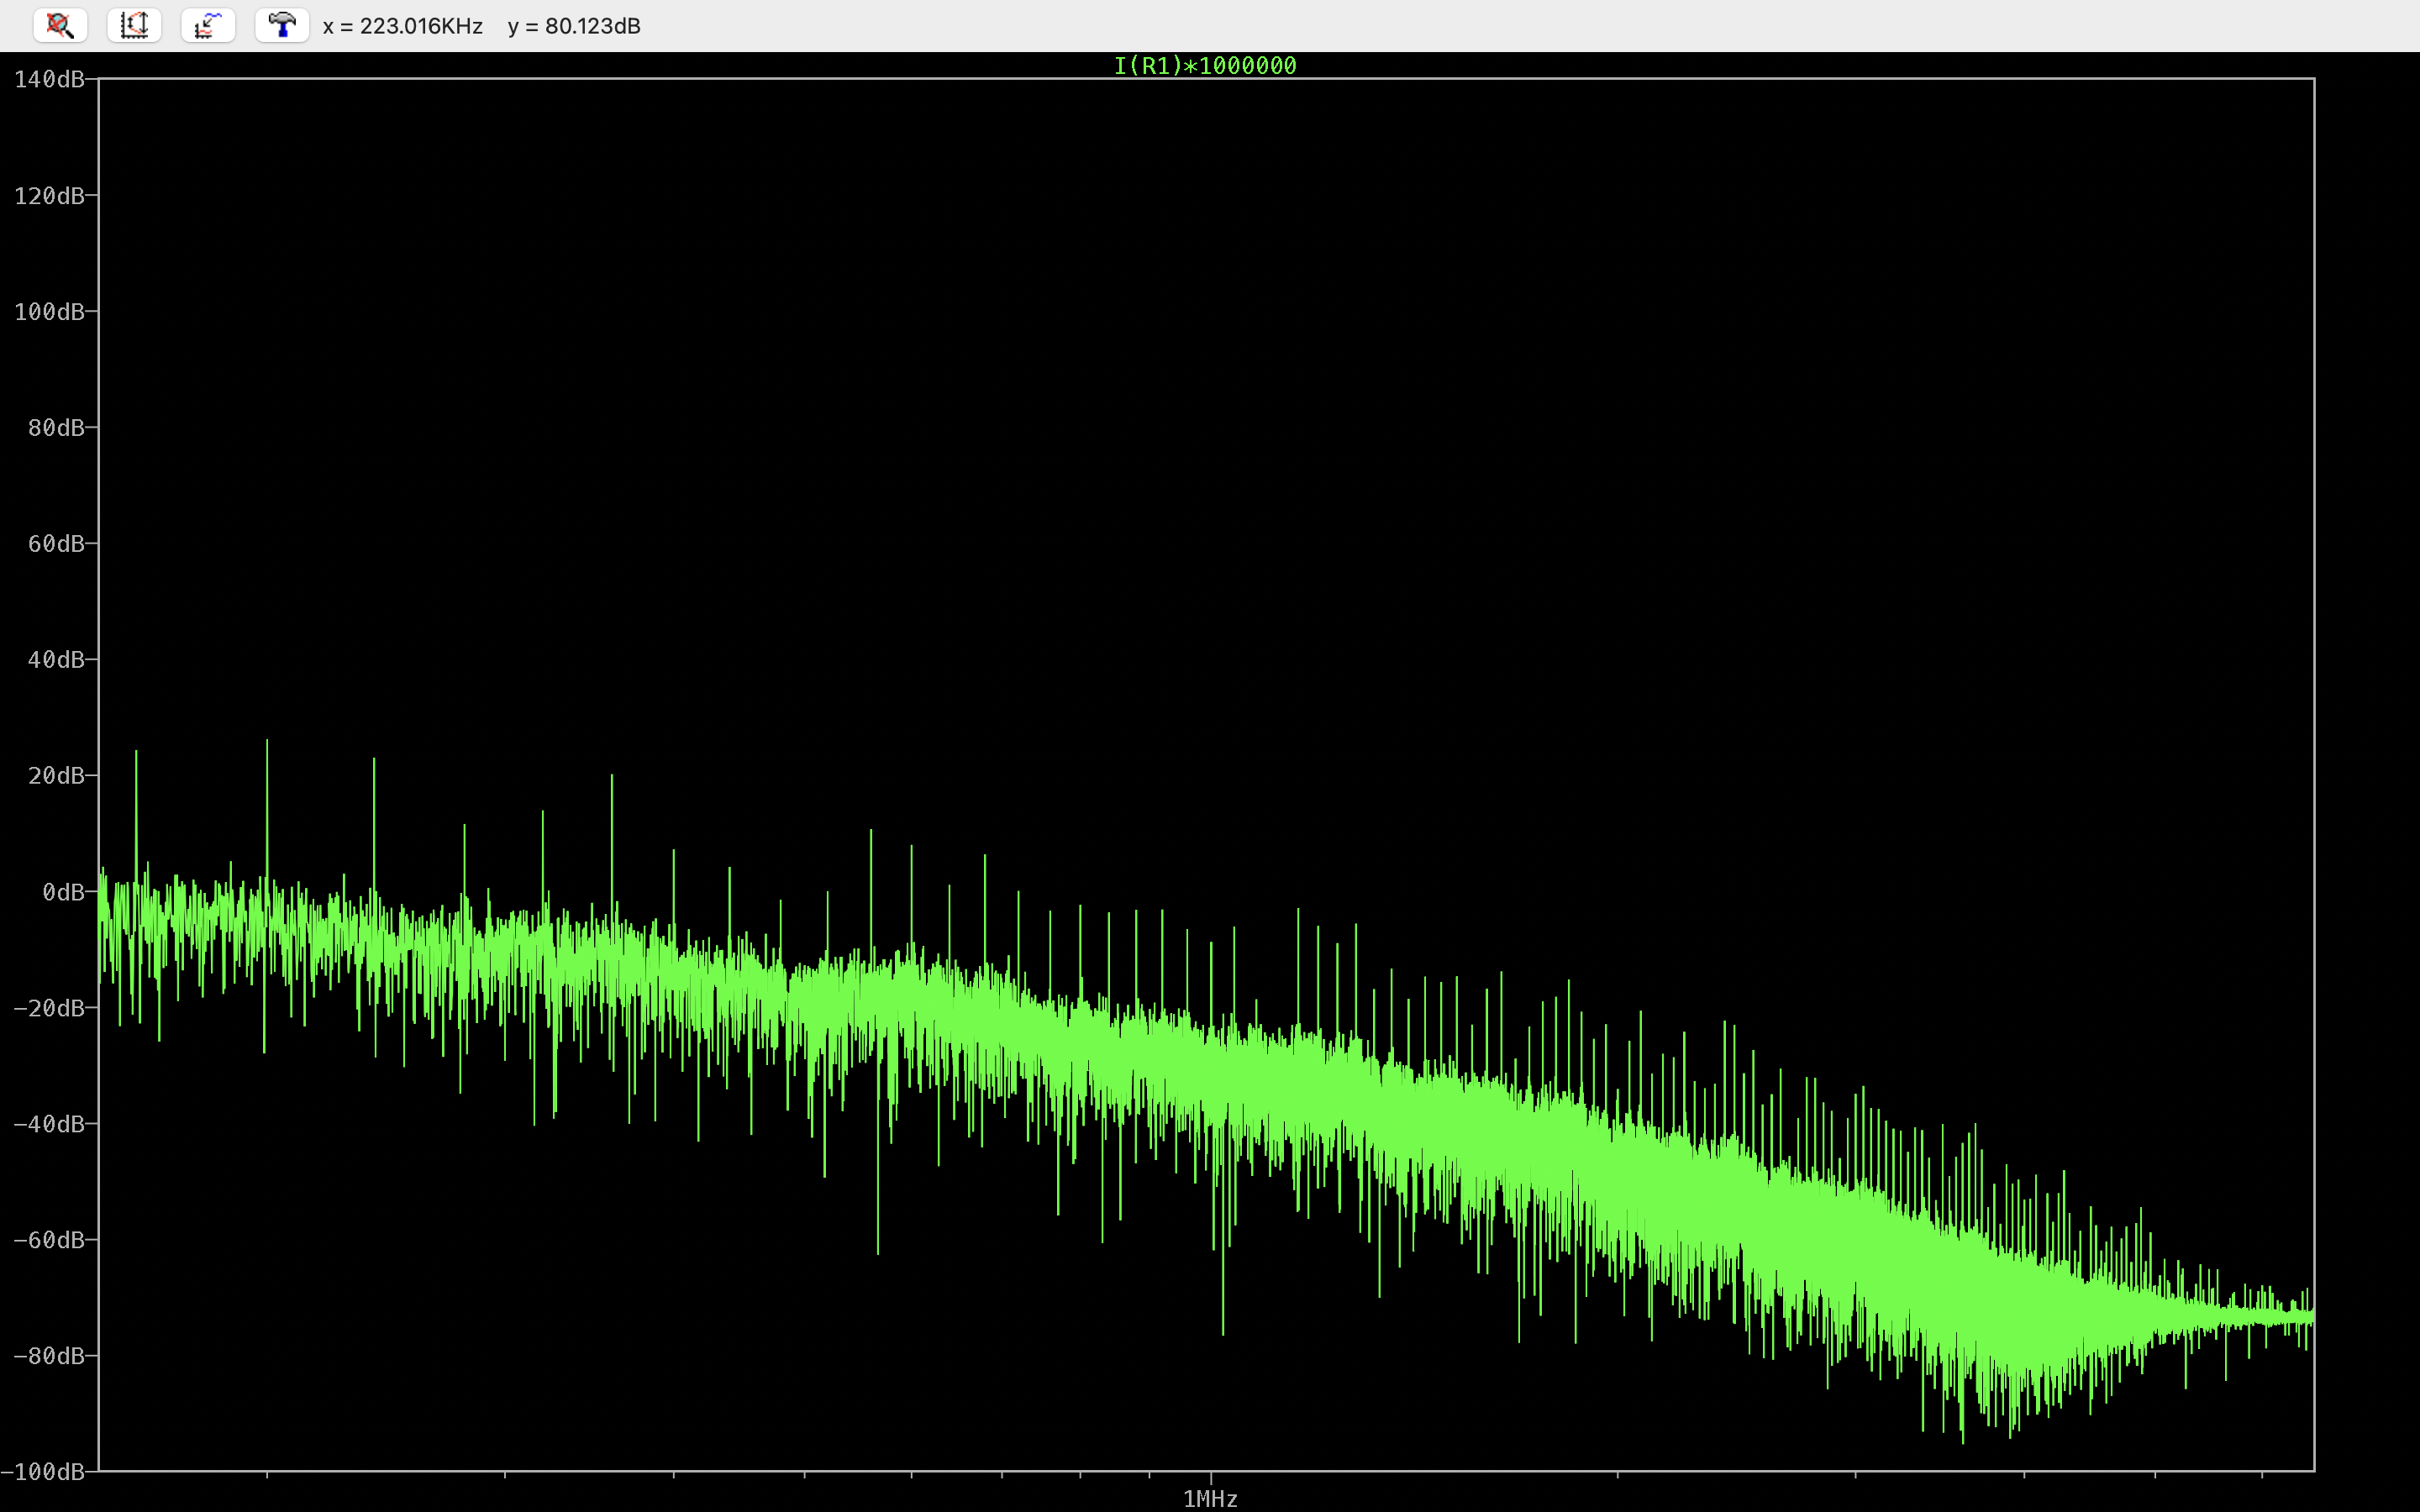
\includegraphics[width=1.0\linewidth]{load_fft_150kHz_16MHz.png}
    \caption{FFT of current (dBuA) across load from 150$kHz$ to 16.55$MHz$ frequency range}
    \label{fig:load_fft_150kHz_16MHz_waveform}
\end{figure}

\section{Discussion}
\subsection{Conducted Emissions at the Load}
\subsection{Open Risks and Concerns}

\nocite{*}
\bibliographystyle{ieeetr}
\bibliography{final_project.bib}

\end{document}
